% Options for packages loaded elsewhere
\PassOptionsToPackage{unicode}{hyperref}
\PassOptionsToPackage{hyphens}{url}
%
\documentclass[
]{article}
\usepackage{amsmath,amssymb}
\usepackage{iftex}
\ifPDFTeX
  \usepackage[T1]{fontenc}
  \usepackage[utf8]{inputenc}
  \usepackage{textcomp} % provide euro and other symbols
\else % if luatex or xetex
  \usepackage{unicode-math} % this also loads fontspec
  \defaultfontfeatures{Scale=MatchLowercase}
  \defaultfontfeatures[\rmfamily]{Ligatures=TeX,Scale=1}
\fi
\usepackage{lmodern}
\ifPDFTeX\else
  % xetex/luatex font selection
\fi
% Use upquote if available, for straight quotes in verbatim environments
\IfFileExists{upquote.sty}{\usepackage{upquote}}{}
\IfFileExists{microtype.sty}{% use microtype if available
  \usepackage[]{microtype}
  \UseMicrotypeSet[protrusion]{basicmath} % disable protrusion for tt fonts
}{}
\makeatletter
\@ifundefined{KOMAClassName}{% if non-KOMA class
  \IfFileExists{parskip.sty}{%
    \usepackage{parskip}
  }{% else
    \setlength{\parindent}{0pt}
    \setlength{\parskip}{6pt plus 2pt minus 1pt}}
}{% if KOMA class
  \KOMAoptions{parskip=half}}
\makeatother
\usepackage{xcolor}
\usepackage[margin=1in]{geometry}
\usepackage{color}
\usepackage{fancyvrb}
\newcommand{\VerbBar}{|}
\newcommand{\VERB}{\Verb[commandchars=\\\{\}]}
\DefineVerbatimEnvironment{Highlighting}{Verbatim}{commandchars=\\\{\}}
% Add ',fontsize=\small' for more characters per line
\usepackage{framed}
\definecolor{shadecolor}{RGB}{248,248,248}
\newenvironment{Shaded}{\begin{snugshade}}{\end{snugshade}}
\newcommand{\AlertTok}[1]{\textcolor[rgb]{0.94,0.16,0.16}{#1}}
\newcommand{\AnnotationTok}[1]{\textcolor[rgb]{0.56,0.35,0.01}{\textbf{\textit{#1}}}}
\newcommand{\AttributeTok}[1]{\textcolor[rgb]{0.13,0.29,0.53}{#1}}
\newcommand{\BaseNTok}[1]{\textcolor[rgb]{0.00,0.00,0.81}{#1}}
\newcommand{\BuiltInTok}[1]{#1}
\newcommand{\CharTok}[1]{\textcolor[rgb]{0.31,0.60,0.02}{#1}}
\newcommand{\CommentTok}[1]{\textcolor[rgb]{0.56,0.35,0.01}{\textit{#1}}}
\newcommand{\CommentVarTok}[1]{\textcolor[rgb]{0.56,0.35,0.01}{\textbf{\textit{#1}}}}
\newcommand{\ConstantTok}[1]{\textcolor[rgb]{0.56,0.35,0.01}{#1}}
\newcommand{\ControlFlowTok}[1]{\textcolor[rgb]{0.13,0.29,0.53}{\textbf{#1}}}
\newcommand{\DataTypeTok}[1]{\textcolor[rgb]{0.13,0.29,0.53}{#1}}
\newcommand{\DecValTok}[1]{\textcolor[rgb]{0.00,0.00,0.81}{#1}}
\newcommand{\DocumentationTok}[1]{\textcolor[rgb]{0.56,0.35,0.01}{\textbf{\textit{#1}}}}
\newcommand{\ErrorTok}[1]{\textcolor[rgb]{0.64,0.00,0.00}{\textbf{#1}}}
\newcommand{\ExtensionTok}[1]{#1}
\newcommand{\FloatTok}[1]{\textcolor[rgb]{0.00,0.00,0.81}{#1}}
\newcommand{\FunctionTok}[1]{\textcolor[rgb]{0.13,0.29,0.53}{\textbf{#1}}}
\newcommand{\ImportTok}[1]{#1}
\newcommand{\InformationTok}[1]{\textcolor[rgb]{0.56,0.35,0.01}{\textbf{\textit{#1}}}}
\newcommand{\KeywordTok}[1]{\textcolor[rgb]{0.13,0.29,0.53}{\textbf{#1}}}
\newcommand{\NormalTok}[1]{#1}
\newcommand{\OperatorTok}[1]{\textcolor[rgb]{0.81,0.36,0.00}{\textbf{#1}}}
\newcommand{\OtherTok}[1]{\textcolor[rgb]{0.56,0.35,0.01}{#1}}
\newcommand{\PreprocessorTok}[1]{\textcolor[rgb]{0.56,0.35,0.01}{\textit{#1}}}
\newcommand{\RegionMarkerTok}[1]{#1}
\newcommand{\SpecialCharTok}[1]{\textcolor[rgb]{0.81,0.36,0.00}{\textbf{#1}}}
\newcommand{\SpecialStringTok}[1]{\textcolor[rgb]{0.31,0.60,0.02}{#1}}
\newcommand{\StringTok}[1]{\textcolor[rgb]{0.31,0.60,0.02}{#1}}
\newcommand{\VariableTok}[1]{\textcolor[rgb]{0.00,0.00,0.00}{#1}}
\newcommand{\VerbatimStringTok}[1]{\textcolor[rgb]{0.31,0.60,0.02}{#1}}
\newcommand{\WarningTok}[1]{\textcolor[rgb]{0.56,0.35,0.01}{\textbf{\textit{#1}}}}
\usepackage{graphicx}
\makeatletter
\def\maxwidth{\ifdim\Gin@nat@width>\linewidth\linewidth\else\Gin@nat@width\fi}
\def\maxheight{\ifdim\Gin@nat@height>\textheight\textheight\else\Gin@nat@height\fi}
\makeatother
% Scale images if necessary, so that they will not overflow the page
% margins by default, and it is still possible to overwrite the defaults
% using explicit options in \includegraphics[width, height, ...]{}
\setkeys{Gin}{width=\maxwidth,height=\maxheight,keepaspectratio}
% Set default figure placement to htbp
\makeatletter
\def\fps@figure{htbp}
\makeatother
\setlength{\emergencystretch}{3em} % prevent overfull lines
\providecommand{\tightlist}{%
  \setlength{\itemsep}{0pt}\setlength{\parskip}{0pt}}
\setcounter{secnumdepth}{-\maxdimen} % remove section numbering
\ifLuaTeX
  \usepackage{selnolig}  % disable illegal ligatures
\fi
\IfFileExists{bookmark.sty}{\usepackage{bookmark}}{\usepackage{hyperref}}
\IfFileExists{xurl.sty}{\usepackage{xurl}}{} % add URL line breaks if available
\urlstyle{same}
\hypersetup{
  pdftitle={Analysis of the DSTP parameters},
  pdfauthor={corrado},
  hidelinks,
  pdfcreator={LaTeX via pandoc}}

\title{Analysis of the DSTP parameters}
\author{corrado}
\date{2023-09-20}

\begin{document}
\maketitle

\begin{Shaded}
\begin{Highlighting}[]
\FunctionTok{library}\NormalTok{(}\StringTok{"here"}\NormalTok{)}
\end{Highlighting}
\end{Shaded}

\begin{verbatim}
## here() starts at /Users/corrado/_repositories/surprise
\end{verbatim}

\begin{Shaded}
\begin{Highlighting}[]
\FunctionTok{suppressPackageStartupMessages}\NormalTok{(\{}
  \FunctionTok{library}\NormalTok{(}\StringTok{"tidyverse"}\NormalTok{)}
  \FunctionTok{library}\NormalTok{(}\StringTok{"brms"}\NormalTok{)}
  \FunctionTok{library}\NormalTok{(}\StringTok{"cmdstanr"}\NormalTok{)}
  \FunctionTok{library}\NormalTok{(}\StringTok{"mice"}\NormalTok{)}
  \FunctionTok{library}\NormalTok{(}\StringTok{"tidybayes"}\NormalTok{)}
  \FunctionTok{library}\NormalTok{(}\StringTok{"emmeans"}\NormalTok{)}
  \FunctionTok{library}\NormalTok{(}\StringTok{"broom.mixed"}\NormalTok{)}
  \FunctionTok{library}\NormalTok{(}\StringTok{"patchwork"}\NormalTok{)}
\NormalTok{\})}

\FunctionTok{theme\_set}\NormalTok{(bayesplot}\SpecialCharTok{::}\FunctionTok{theme\_default}\NormalTok{(}\AttributeTok{base\_family =} \StringTok{"sans"}\NormalTok{, }\AttributeTok{base\_size =} \DecValTok{14}\NormalTok{))}
\FunctionTok{set.seed}\NormalTok{(}\DecValTok{123}\NormalTok{)}

\NormalTok{params\_cntl }\OtherTok{\textless{}{-}}\NormalTok{ rio}\SpecialCharTok{::}\FunctionTok{import}\NormalTok{(}
\NormalTok{  here}\SpecialCharTok{::}\FunctionTok{here}\NormalTok{(}
    \StringTok{"data"}\NormalTok{, }\StringTok{"processed"}\NormalTok{, }\StringTok{"params\_data"}\NormalTok{, }\StringTok{"dstp"}\NormalTok{, }\StringTok{"control\_DSTP\_params.csv"}
\NormalTok{  )}
\NormalTok{)}
\NormalTok{params\_cntl}\SpecialCharTok{$}\NormalTok{exp }\OtherTok{\textless{}{-}} \StringTok{"control"}

\NormalTok{params\_surprise }\OtherTok{\textless{}{-}}\NormalTok{ rio}\SpecialCharTok{::}\FunctionTok{import}\NormalTok{(}
\NormalTok{  here}\SpecialCharTok{::}\FunctionTok{here}\NormalTok{(}
    \StringTok{"data"}\NormalTok{, }\StringTok{"processed"}\NormalTok{, }\StringTok{"params\_data"}\NormalTok{, }\StringTok{"dstp"}\NormalTok{, }\StringTok{"surprise\_DSTP\_params.csv"}
\NormalTok{  )}
\NormalTok{)}
\NormalTok{params\_surprise}\SpecialCharTok{$}\NormalTok{exp }\OtherTok{\textless{}{-}} \StringTok{"surprise"}
\CommentTok{\# In both experiments, the subjects\textquotesingle{} id start from 1.}
\NormalTok{params\_surprise}\SpecialCharTok{$}\NormalTok{subject }\OtherTok{\textless{}{-}}\NormalTok{ params\_surprise}\SpecialCharTok{$}\NormalTok{subject }\SpecialCharTok{+} \DecValTok{500}

\NormalTok{df }\OtherTok{\textless{}{-}} \FunctionTok{bind\_rows}\NormalTok{(params\_cntl, params\_surprise)}
\NormalTok{df}\SpecialCharTok{$}\NormalTok{blk }\OtherTok{\textless{}{-}} \FunctionTok{factor}\NormalTok{(df}\SpecialCharTok{$}\NormalTok{block)}
\end{Highlighting}
\end{Shaded}

\hypertarget{parameter-a}{%
\section{Parameter A:}\label{parameter-a}}

Height of the boundary for the response selection diffusion process

\begin{Shaded}
\begin{Highlighting}[]
\NormalTok{m1 }\OtherTok{\textless{}{-}} \FunctionTok{brm}\NormalTok{(}
\NormalTok{  A }\SpecialCharTok{\textasciitilde{}}\NormalTok{ exp }\SpecialCharTok{*}\NormalTok{ blk }\SpecialCharTok{+}\NormalTok{ (}\DecValTok{1} \SpecialCharTok{+}\NormalTok{ blk }\SpecialCharTok{|}\NormalTok{ subject),}
  \AttributeTok{family =} \FunctionTok{shifted\_lognormal}\NormalTok{(),}
  \AttributeTok{backend =} \StringTok{"cmdstanr"}\NormalTok{,}
  \AttributeTok{data =}\NormalTok{ df}
\NormalTok{)}
\end{Highlighting}
\end{Shaded}

\begin{verbatim}
## In file included from /var/folders/cl/wwjrsxdd5tz7y9jr82nd5hrw0000gn/T/RtmpDVAVEa/model-d44073536660.hpp:1:
## In file included from /Users/corrado/.cmdstan/cmdstan-2.33.1/stan/src/stan/model/model_header.hpp:4:
## In file included from /Users/corrado/.cmdstan/cmdstan-2.33.1/stan/lib/stan_math/stan/math.hpp:19:
## In file included from /Users/corrado/.cmdstan/cmdstan-2.33.1/stan/lib/stan_math/stan/math/rev.hpp:10:
## In file included from /Users/corrado/.cmdstan/cmdstan-2.33.1/stan/lib/stan_math/stan/math/rev/fun.hpp:200:
## In file included from /Users/corrado/.cmdstan/cmdstan-2.33.1/stan/lib/stan_math/stan/math/prim/functor.hpp:16:
## In file included from /Users/corrado/.cmdstan/cmdstan-2.33.1/stan/lib/stan_math/stan/math/prim/functor/integrate_ode_rk45.hpp:6:
## In file included from /Users/corrado/.cmdstan/cmdstan-2.33.1/stan/lib/stan_math/stan/math/prim/functor/ode_rk45.hpp:9:
## In file included from /Users/corrado/.cmdstan/cmdstan-2.33.1/stan/lib/stan_math/lib/boost_1.78.0/boost/numeric/odeint.hpp:76:
## In file included from /Users/corrado/.cmdstan/cmdstan-2.33.1/stan/lib/stan_math/lib/boost_1.78.0/boost/numeric/odeint/integrate/observer_collection.hpp:23:
## In file included from /Users/corrado/.cmdstan/cmdstan-2.33.1/stan/lib/stan_math/lib/boost_1.78.0/boost/function.hpp:30:
## In file included from /Users/corrado/.cmdstan/cmdstan-2.33.1/stan/lib/stan_math/lib/boost_1.78.0/boost/function/detail/prologue.hpp:17:
## In file included from /Users/corrado/.cmdstan/cmdstan-2.33.1/stan/lib/stan_math/lib/boost_1.78.0/boost/function/function_base.hpp:21:
## In file included from /Users/corrado/.cmdstan/cmdstan-2.33.1/stan/lib/stan_math/lib/boost_1.78.0/boost/type_index.hpp:29:
## In file included from /Users/corrado/.cmdstan/cmdstan-2.33.1/stan/lib/stan_math/lib/boost_1.78.0/boost/type_index/stl_type_index.hpp:47:
## /Users/corrado/.cmdstan/cmdstan-2.33.1/stan/lib/stan_math/lib/boost_1.78.0/boost/container_hash/hash.hpp:132:33: warning: 'unary_function<const std::error_category *, unsigned long>' is deprecat
\end{verbatim}

\begin{verbatim}
## ed [-Wdeprecated-declarations]
##         struct hash_base : std::unary_function<T, std::size_t> {};
##                                 ^
\end{verbatim}

\begin{verbatim}
## /Users/corrado/.cmdstan/cmdstan-2.33.1/stan/lib/stan_math/lib/boost_1.78.0/boost/container_hash/hash.hpp:692:18: note: in instantiation of template class 'boost::hash_detail::hash_base<const std::error_category *>' requested here
##         : public boost::hash_detail::hash_base<T*>
##                  ^
## /Users/corrado/.cmdstan/cmdstan-2.33.1/stan/lib/stan_math/lib/boost_1.78.0/boost/container_hash/hash.hpp:420:24: note: in instantiation of template class 'boost::hash<const std::error_category *>' requested here
##         boost::hash<T> hasher;
##                        ^
## /Users/corrado/.cmdstan/cmdstan-2.33.1/stan/lib/stan_math/lib/boost_1.78.0/boost/container_hash/hash.hpp:551:9: note: in instantiation of function template specialization 'boost::hash_combine<const std::error_category *>' requested here
##         hash_combine(seed, &v.category());
##         ^
## /Library/Developer/CommandLineTools/SDKs/MacOSX.sdk/usr/include/c++/v1/__functional/unary_function.h:23:29: note: 'unary_function<const std::error_category *, unsigned long>' has been explicitly marked deprecated here
## struct _LIBCPP_TEMPLATE_VIS _LIBCPP_DEPRECATED_IN_CXX11 unary_function
##                             ^
## /Library/Developer/CommandLineTools/SDKs/MacOSX.sdk/usr/include/c++/v1/__config:825:41: note: expanded from macro '_LIBCPP_DEPRECATED_IN_CXX11'
## #    define _LIBCPP_DEPRECATED_IN_CXX11 _LIBCPP_DEPRECATED
##                                         ^
## /Library/Developer/CommandLineTools/SDKs/MacOSX.sdk/usr/include/c++/v1/__config:810:49: note: expanded from macro '_LIBCPP_DEPRECATED'
## #      define _LIBCPP_DEPRECATED __attribute__((deprecated))
##                                                 ^
\end{verbatim}

\begin{verbatim}
## 1 warning generated.
\end{verbatim}

\begin{verbatim}
## Start sampling
\end{verbatim}

\begin{verbatim}
## Running MCMC with 4 sequential chains...
## 
## Chain 1 Iteration:    1 / 2000 [  0%]  (Warmup) 
## Chain 1 Iteration:  100 / 2000 [  5%]  (Warmup) 
## Chain 1 Iteration:  200 / 2000 [ 10%]  (Warmup) 
## Chain 1 Iteration:  300 / 2000 [ 15%]  (Warmup) 
## Chain 1 Iteration:  400 / 2000 [ 20%]  (Warmup) 
## Chain 1 Iteration:  500 / 2000 [ 25%]  (Warmup) 
## Chain 1 Iteration:  600 / 2000 [ 30%]  (Warmup) 
## Chain 1 Iteration:  700 / 2000 [ 35%]  (Warmup) 
## Chain 1 Iteration:  800 / 2000 [ 40%]  (Warmup) 
## Chain 1 Iteration:  900 / 2000 [ 45%]  (Warmup) 
## Chain 1 Iteration: 1000 / 2000 [ 50%]  (Warmup) 
## Chain 1 Iteration: 1001 / 2000 [ 50%]  (Sampling) 
## Chain 1 Iteration: 1100 / 2000 [ 55%]  (Sampling) 
## Chain 1 Iteration: 1200 / 2000 [ 60%]  (Sampling) 
## Chain 1 Iteration: 1300 / 2000 [ 65%]  (Sampling) 
## Chain 1 Iteration: 1400 / 2000 [ 70%]  (Sampling) 
## Chain 1 Iteration: 1500 / 2000 [ 75%]  (Sampling) 
## Chain 1 Iteration: 1600 / 2000 [ 80%]  (Sampling) 
## Chain 1 Iteration: 1700 / 2000 [ 85%]  (Sampling) 
## Chain 1 Iteration: 1800 / 2000 [ 90%]  (Sampling) 
## Chain 1 Iteration: 1900 / 2000 [ 95%]  (Sampling) 
## Chain 1 Iteration: 2000 / 2000 [100%]  (Sampling) 
## Chain 1 finished in 7.1 seconds.
## Chain 2 Iteration:    1 / 2000 [  0%]  (Warmup) 
## Chain 2 Iteration:  100 / 2000 [  5%]  (Warmup) 
## Chain 2 Iteration:  200 / 2000 [ 10%]  (Warmup) 
## Chain 2 Iteration:  300 / 2000 [ 15%]  (Warmup) 
## Chain 2 Iteration:  400 / 2000 [ 20%]  (Warmup) 
## Chain 2 Iteration:  500 / 2000 [ 25%]  (Warmup) 
## Chain 2 Iteration:  600 / 2000 [ 30%]  (Warmup) 
## Chain 2 Iteration:  700 / 2000 [ 35%]  (Warmup) 
## Chain 2 Iteration:  800 / 2000 [ 40%]  (Warmup) 
## Chain 2 Iteration:  900 / 2000 [ 45%]  (Warmup) 
## Chain 2 Iteration: 1000 / 2000 [ 50%]  (Warmup) 
## Chain 2 Iteration: 1001 / 2000 [ 50%]  (Sampling) 
## Chain 2 Iteration: 1100 / 2000 [ 55%]  (Sampling) 
## Chain 2 Iteration: 1200 / 2000 [ 60%]  (Sampling) 
## Chain 2 Iteration: 1300 / 2000 [ 65%]  (Sampling) 
## Chain 2 Iteration: 1400 / 2000 [ 70%]  (Sampling) 
## Chain 2 Iteration: 1500 / 2000 [ 75%]  (Sampling) 
## Chain 2 Iteration: 1600 / 2000 [ 80%]  (Sampling) 
## Chain 2 Iteration: 1700 / 2000 [ 85%]  (Sampling) 
## Chain 2 Iteration: 1800 / 2000 [ 90%]  (Sampling) 
## Chain 2 Iteration: 1900 / 2000 [ 95%]  (Sampling) 
## Chain 2 Iteration: 2000 / 2000 [100%]  (Sampling) 
## Chain 2 finished in 7.0 seconds.
## Chain 3 Iteration:    1 / 2000 [  0%]  (Warmup) 
## Chain 3 Iteration:  100 / 2000 [  5%]  (Warmup) 
## Chain 3 Iteration:  200 / 2000 [ 10%]  (Warmup) 
## Chain 3 Iteration:  300 / 2000 [ 15%]  (Warmup) 
## Chain 3 Iteration:  400 / 2000 [ 20%]  (Warmup) 
## Chain 3 Iteration:  500 / 2000 [ 25%]  (Warmup) 
## Chain 3 Iteration:  600 / 2000 [ 30%]  (Warmup) 
## Chain 3 Iteration:  700 / 2000 [ 35%]  (Warmup) 
## Chain 3 Iteration:  800 / 2000 [ 40%]  (Warmup) 
## Chain 3 Iteration:  900 / 2000 [ 45%]  (Warmup) 
## Chain 3 Iteration: 1000 / 2000 [ 50%]  (Warmup) 
## Chain 3 Iteration: 1001 / 2000 [ 50%]  (Sampling) 
## Chain 3 Iteration: 1100 / 2000 [ 55%]  (Sampling) 
## Chain 3 Iteration: 1200 / 2000 [ 60%]  (Sampling) 
## Chain 3 Iteration: 1300 / 2000 [ 65%]  (Sampling) 
## Chain 3 Iteration: 1400 / 2000 [ 70%]  (Sampling) 
## Chain 3 Iteration: 1500 / 2000 [ 75%]  (Sampling) 
## Chain 3 Iteration: 1600 / 2000 [ 80%]  (Sampling) 
## Chain 3 Iteration: 1700 / 2000 [ 85%]  (Sampling) 
## Chain 3 Iteration: 1800 / 2000 [ 90%]  (Sampling) 
## Chain 3 Iteration: 1900 / 2000 [ 95%]  (Sampling) 
## Chain 3 Iteration: 2000 / 2000 [100%]  (Sampling) 
## Chain 3 finished in 7.5 seconds.
## Chain 4 Iteration:    1 / 2000 [  0%]  (Warmup) 
## Chain 4 Iteration:  100 / 2000 [  5%]  (Warmup) 
## Chain 4 Iteration:  200 / 2000 [ 10%]  (Warmup) 
## Chain 4 Iteration:  300 / 2000 [ 15%]  (Warmup) 
## Chain 4 Iteration:  400 / 2000 [ 20%]  (Warmup) 
## Chain 4 Iteration:  500 / 2000 [ 25%]  (Warmup) 
## Chain 4 Iteration:  600 / 2000 [ 30%]  (Warmup) 
## Chain 4 Iteration:  700 / 2000 [ 35%]  (Warmup) 
## Chain 4 Iteration:  800 / 2000 [ 40%]  (Warmup) 
## Chain 4 Iteration:  900 / 2000 [ 45%]  (Warmup) 
## Chain 4 Iteration: 1000 / 2000 [ 50%]  (Warmup) 
## Chain 4 Iteration: 1001 / 2000 [ 50%]  (Sampling) 
## Chain 4 Iteration: 1100 / 2000 [ 55%]  (Sampling) 
## Chain 4 Iteration: 1200 / 2000 [ 60%]  (Sampling) 
## Chain 4 Iteration: 1300 / 2000 [ 65%]  (Sampling) 
## Chain 4 Iteration: 1400 / 2000 [ 70%]  (Sampling) 
## Chain 4 Iteration: 1500 / 2000 [ 75%]  (Sampling) 
## Chain 4 Iteration: 1600 / 2000 [ 80%]  (Sampling) 
## Chain 4 Iteration: 1700 / 2000 [ 85%]  (Sampling) 
## Chain 4 Iteration: 1800 / 2000 [ 90%]  (Sampling) 
## Chain 4 Iteration: 1900 / 2000 [ 95%]  (Sampling) 
## Chain 4 Iteration: 2000 / 2000 [100%]  (Sampling) 
## Chain 4 finished in 7.1 seconds.
## 
## All 4 chains finished successfully.
## Mean chain execution time: 7.2 seconds.
## Total execution time: 29.0 seconds.
\end{verbatim}

\begin{verbatim}
## Warning: 4 of 4 chains had an E-BFMI less than 0.2.
## See https://mc-stan.org/misc/warnings for details.
\end{verbatim}

\begin{Shaded}
\begin{Highlighting}[]
\FunctionTok{pp\_check}\NormalTok{(m1)}
\end{Highlighting}
\end{Shaded}

\begin{verbatim}
## Using 10 posterior draws for ppc type 'dens_overlay' by default.
\end{verbatim}

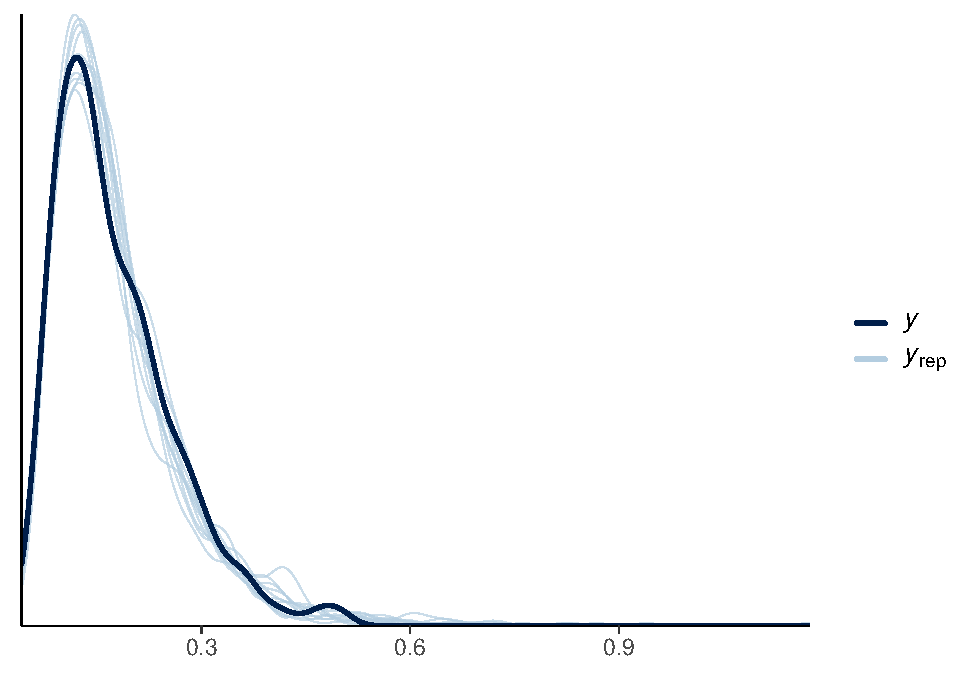
\includegraphics{params_analyses_files/figure-latex/unnamed-chunk-2-1.pdf}

\begin{Shaded}
\begin{Highlighting}[]
\FunctionTok{summary}\NormalTok{(m1)}
\end{Highlighting}
\end{Shaded}

\begin{verbatim}
## Warning: Parts of the model have not converged (some Rhats are > 1.05). Be
## careful when analysing the results! We recommend running more iterations and/or
## setting stronger priors.
\end{verbatim}

\begin{verbatim}
##  Family: shifted_lognormal 
##   Links: mu = identity; sigma = identity; ndt = identity 
## Formula: A ~ exp * blk + (1 + blk | subject) 
##    Data: df (Number of observations: 736) 
##   Draws: 4 chains, each with iter = 2000; warmup = 1000; thin = 1;
##          total post-warmup draws = 4000
## 
## Group-Level Effects: 
## ~subject (Number of levels: 184) 
##                     Estimate Est.Error l-95% CI u-95% CI Rhat Bulk_ESS Tail_ESS
## sd(Intercept)           0.52      0.05     0.42     0.63 1.09       34      112
## sd(blk2)                0.46      0.08     0.31     0.63 1.14       20       31
## sd(blk3)                0.49      0.08     0.35     0.66 1.13       22       33
## sd(blk4)                0.56      0.08     0.42     0.73 1.12       25       37
## cor(Intercept,blk2)    -0.47      0.10    -0.64    -0.24 1.03      156     1302
## cor(Intercept,blk3)    -0.50      0.09    -0.66    -0.30 1.03      158     1567
## cor(blk2,blk3)          0.83      0.08     0.68     0.97 1.08       39      761
## cor(Intercept,blk4)    -0.56      0.08    -0.69    -0.39 1.02      287     1787
## cor(blk2,blk4)          0.79      0.08     0.62     0.95 1.06       50      516
## cor(blk3,blk4)          0.89      0.06     0.76     0.99 1.12       24       66
## 
## Population-Level Effects: 
##                  Estimate Est.Error l-95% CI u-95% CI Rhat Bulk_ESS Tail_ESS
## Intercept           -2.15      0.08    -2.31    -1.99 1.00     1124     1471
## expsurprise          0.11      0.09    -0.07     0.29 1.00     1064     1659
## blk2                 0.00      0.08    -0.14     0.15 1.00     1181     1779
## blk3                -0.05      0.08    -0.20     0.11 1.00     1153     1629
## blk4                -0.07      0.09    -0.23     0.10 1.00     1053     1468
## expsurprise:blk2     0.02      0.10    -0.17     0.21 1.00     1136     1737
## expsurprise:blk3     0.04      0.10    -0.16     0.23 1.00     1168     1963
## expsurprise:blk4     0.03      0.11    -0.19     0.24 1.00     1111     1662
## 
## Family Specific Parameters: 
##       Estimate Est.Error l-95% CI u-95% CI Rhat Bulk_ESS Tail_ESS
## sigma     0.32      0.05     0.19     0.39 1.19       15       19
## ndt       0.03      0.00     0.02     0.04 1.00     2017     2192
## 
## Draws were sampled using sample(hmc). For each parameter, Bulk_ESS
## and Tail_ESS are effective sample size measures, and Rhat is the potential
## scale reduction factor on split chains (at convergence, Rhat = 1).
\end{verbatim}

\begin{Shaded}
\begin{Highlighting}[]
\FunctionTok{conditional\_effects}\NormalTok{(m1, }\StringTok{"blk:exp"}\NormalTok{)}
\end{Highlighting}
\end{Shaded}

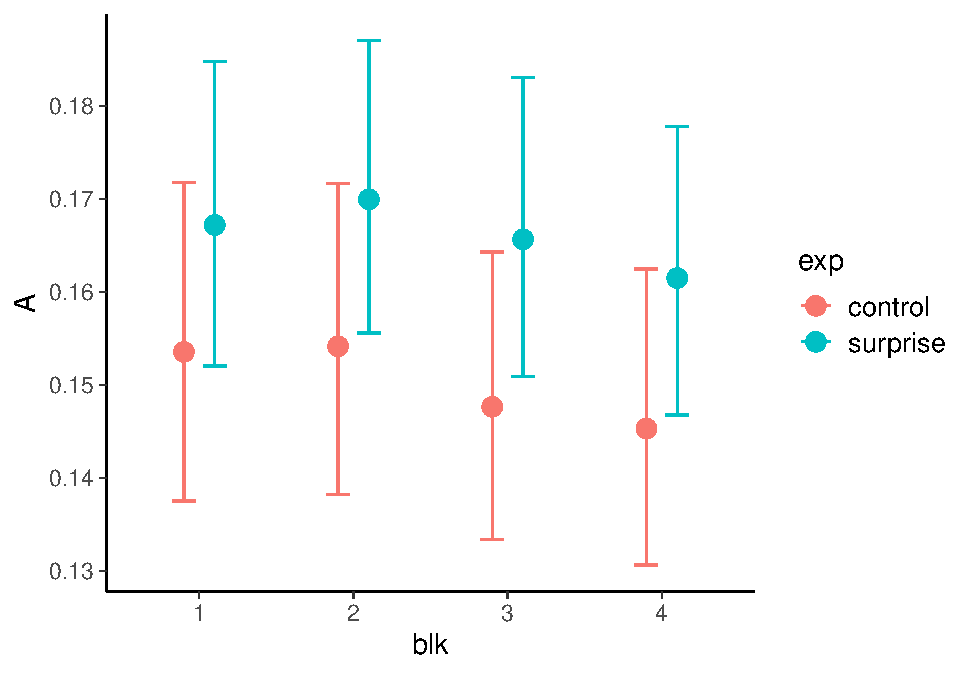
\includegraphics{params_analyses_files/figure-latex/unnamed-chunk-2-2.pdf}

Parameter C: Height of the boundary for the stimulus selection diffusion
process

\begin{Shaded}
\begin{Highlighting}[]
\FunctionTok{hist}\NormalTok{(df}\SpecialCharTok{$}\NormalTok{C)}
\end{Highlighting}
\end{Shaded}

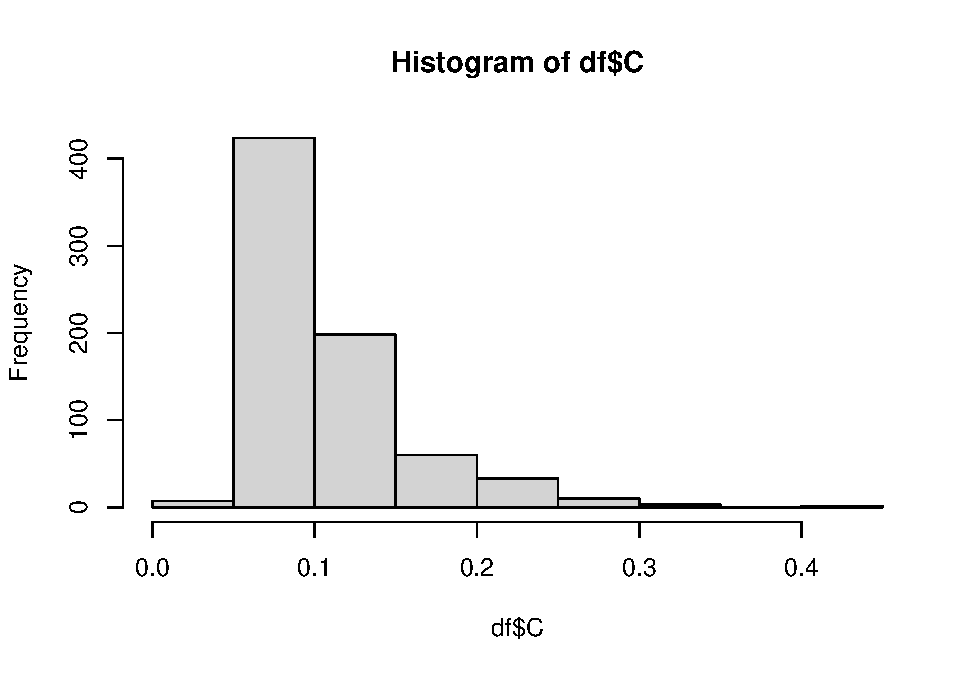
\includegraphics{params_analyses_files/figure-latex/unnamed-chunk-3-1.pdf}

\begin{Shaded}
\begin{Highlighting}[]
\NormalTok{m2 }\OtherTok{\textless{}{-}} \FunctionTok{brm}\NormalTok{(}
\NormalTok{  C }\SpecialCharTok{\textasciitilde{}}\NormalTok{ exp }\SpecialCharTok{*}\NormalTok{ blk }\SpecialCharTok{+}\NormalTok{ (}\DecValTok{1} \SpecialCharTok{+}\NormalTok{ blk }\SpecialCharTok{|}\NormalTok{ subject),}
  \AttributeTok{family =} \FunctionTok{shifted\_lognormal}\NormalTok{(),}
  \AttributeTok{backend =} \StringTok{"cmdstanr"}\NormalTok{,}
  \CommentTok{\# algorithm = "meanfield",}
  \AttributeTok{data =}\NormalTok{ df}
\NormalTok{)}
\end{Highlighting}
\end{Shaded}

\begin{verbatim}
## In file included from /var/folders/cl/wwjrsxdd5tz7y9jr82nd5hrw0000gn/T/RtmpDVAVEa/model-d44059b7cd9e.hpp:1:
## In file included from /Users/corrado/.cmdstan/cmdstan-2.33.1/stan/src/stan/model/model_header.hpp:4:
## In file included from /Users/corrado/.cmdstan/cmdstan-2.33.1/stan/lib/stan_math/stan/math.hpp:19:
## In file included from /Users/corrado/.cmdstan/cmdstan-2.33.1/stan/lib/stan_math/stan/math/rev.hpp:10:
## In file included from /Users/corrado/.cmdstan/cmdstan-2.33.1/stan/lib/stan_math/stan/math/rev/fun.hpp:200:
## In file included from /Users/corrado/.cmdstan/cmdstan-2.33.1/stan/lib/stan_math/stan/math/prim/functor.hpp:16:
## In file included from /Users/corrado/.cmdstan/cmdstan-2.33.1/stan/lib/stan_math/stan/math/prim/functor/integrate_ode_rk45.hpp:6:
## In file included from /Users/corrado/.cmdstan/cmdstan-2.33.1/stan/lib/stan_math/stan/math/prim/functor/ode_rk45.hpp:9:
## In file included from /Users/corrado/.cmdstan/cmdstan-2.33.1/stan/lib/stan_math/lib/boost_1.78.0/boost/numeric/odeint.hpp:76:
## In file included from /Users/corrado/.cmdstan/cmdstan-2.33.1/stan/lib/stan_math/lib/boost_1.78.0/boost/numeric/odeint/integrate/observer_collection.hpp:23:
## In file included from /Users/corrado/.cmdstan/cmdstan-2.33.1/stan/lib/stan_math/lib/boost_1.78.0/boost/function.hpp:30:
## In file included from /Users/corrado/.cmdstan/cmdstan-2.33.1/stan/lib/stan_math/lib/boost_1.78.0/boost/function/detail/prologue.hpp:17:
## In file included from /Users/corrado/.cmdstan/cmdstan-2.33.1/stan/lib/stan_math/lib/boost_1.78.0/boost/function/function_base.hpp:21:
## In file included from /Users/corrado/.cmdstan/cmdstan-2.33.1/stan/lib/stan_math/lib/boost_1.78.0/boost/type_index.hpp:29:
## In file included from /Users/corrado/.cmdstan/cmdstan-2.33.1/stan/lib/stan_math/lib/boost_1.78.0/boost/type_index/stl_type_index.hpp:47:
## /Users/corrado/.cmdstan/cmdstan-2.33.1/stan/lib/stan_math/lib/boost_1.78.0/boost/container_hash/hash.hpp:132:33: warning: 'unary_function<const std::error_category *, unsigned long>' is deprecat
\end{verbatim}

\begin{verbatim}
## ed [-Wdeprecated-declarations]
##         struct hash_base : std::unary_function<T, std::size_t> {};
##                                 ^
## /Users/corrado/.cmdstan/cmdstan-2.33.1/stan/lib/stan_math/lib/boost_1.78.0/boost/container_hash/hash.hpp:692:18: note: in instantiation of template class 'boost::hash_detail::hash_base<const std::error_category *>' requested here
##         : public boost::hash_detail::hash_base<T*>
##                  ^
## /Users/corrado/.cmdstan/cmdstan-2.33.1/stan/lib/stan_math/lib/boost_1.78.0/boost/container_hash/hash.hpp:420:24: note: in instantiation of template class 'boost::hash<const std::error_category *>' requested here
##         boost::hash<T> hasher;
##                        ^
## /Users/corrado/.cmdstan/cmdstan-2.33.1/stan/lib/stan_math/lib/boost_1.78.0/boost/container_hash/hash.hpp:551:9: note: in instantiation of function template specialization 'boost::hash_combine<const std::error_category *>' requested here
##         hash_combine(seed, &v.category());
##         ^
\end{verbatim}

\begin{verbatim}
## /Library/Developer/CommandLineTools/SDKs/MacOSX.sdk/usr/include/c++/v1/__functional/unary_function.h:23:29: note: 'unary_function<const std::error_category *, unsigned long>' has been explicitly marked deprecated here
## struct _LIBCPP_TEMPLATE_VIS _LIBCPP_DEPRECATED_IN_CXX11 unary_function
##                             ^
## /Library/Developer/CommandLineTools/SDKs/MacOSX.sdk/usr/include/c++/v1/__config:825:41: note: expanded from macro '_LIBCPP_DEPRECATED_IN_CXX11'
## #    define _LIBCPP_DEPRECATED_IN_CXX11 _LIBCPP_DEPRECATED
##                                         ^
## /Library/Developer/CommandLineTools/SDKs/MacOSX.sdk/usr/include/c++/v1/__config:810:49: note: expanded from macro '_LIBCPP_DEPRECATED'
## #      define _LIBCPP_DEPRECATED __attribute__((deprecated))
##                                                 ^
\end{verbatim}

\begin{verbatim}
## 1 warning generated.
\end{verbatim}

\begin{verbatim}
## Start sampling
\end{verbatim}

\begin{verbatim}
## Running MCMC with 4 sequential chains...
## 
## Chain 1 Iteration:    1 / 2000 [  0%]  (Warmup) 
## Chain 1 Iteration:  100 / 2000 [  5%]  (Warmup) 
## Chain 1 Iteration:  200 / 2000 [ 10%]  (Warmup) 
## Chain 1 Iteration:  300 / 2000 [ 15%]  (Warmup) 
## Chain 1 Iteration:  400 / 2000 [ 20%]  (Warmup) 
## Chain 1 Iteration:  500 / 2000 [ 25%]  (Warmup) 
## Chain 1 Iteration:  600 / 2000 [ 30%]  (Warmup) 
## Chain 1 Iteration:  700 / 2000 [ 35%]  (Warmup) 
## Chain 1 Iteration:  800 / 2000 [ 40%]  (Warmup) 
## Chain 1 Iteration:  900 / 2000 [ 45%]  (Warmup) 
## Chain 1 Iteration: 1000 / 2000 [ 50%]  (Warmup) 
## Chain 1 Iteration: 1001 / 2000 [ 50%]  (Sampling) 
## Chain 1 Iteration: 1100 / 2000 [ 55%]  (Sampling) 
## Chain 1 Iteration: 1200 / 2000 [ 60%]  (Sampling) 
## Chain 1 Iteration: 1300 / 2000 [ 65%]  (Sampling) 
## Chain 1 Iteration: 1400 / 2000 [ 70%]  (Sampling) 
## Chain 1 Iteration: 1500 / 2000 [ 75%]  (Sampling) 
## Chain 1 Iteration: 1600 / 2000 [ 80%]  (Sampling) 
## Chain 1 Iteration: 1700 / 2000 [ 85%]  (Sampling) 
## Chain 1 Iteration: 1800 / 2000 [ 90%]  (Sampling) 
## Chain 1 Iteration: 1900 / 2000 [ 95%]  (Sampling) 
## Chain 1 Iteration: 2000 / 2000 [100%]  (Sampling) 
## Chain 1 finished in 10.4 seconds.
## Chain 2 Iteration:    1 / 2000 [  0%]  (Warmup) 
## Chain 2 Iteration:  100 / 2000 [  5%]  (Warmup) 
## Chain 2 Iteration:  200 / 2000 [ 10%]  (Warmup) 
## Chain 2 Iteration:  300 / 2000 [ 15%]  (Warmup) 
## Chain 2 Iteration:  400 / 2000 [ 20%]  (Warmup) 
## Chain 2 Iteration:  500 / 2000 [ 25%]  (Warmup) 
## Chain 2 Iteration:  600 / 2000 [ 30%]  (Warmup) 
## Chain 2 Iteration:  700 / 2000 [ 35%]  (Warmup) 
## Chain 2 Iteration:  800 / 2000 [ 40%]  (Warmup) 
## Chain 2 Iteration:  900 / 2000 [ 45%]  (Warmup) 
## Chain 2 Iteration: 1000 / 2000 [ 50%]  (Warmup) 
## Chain 2 Iteration: 1001 / 2000 [ 50%]  (Sampling) 
## Chain 2 Iteration: 1100 / 2000 [ 55%]  (Sampling) 
## Chain 2 Iteration: 1200 / 2000 [ 60%]  (Sampling) 
## Chain 2 Iteration: 1300 / 2000 [ 65%]  (Sampling) 
## Chain 2 Iteration: 1400 / 2000 [ 70%]  (Sampling) 
## Chain 2 Iteration: 1500 / 2000 [ 75%]  (Sampling) 
## Chain 2 Iteration: 1600 / 2000 [ 80%]  (Sampling) 
## Chain 2 Iteration: 1700 / 2000 [ 85%]  (Sampling) 
## Chain 2 Iteration: 1800 / 2000 [ 90%]  (Sampling) 
## Chain 2 Iteration: 1900 / 2000 [ 95%]  (Sampling) 
## Chain 2 Iteration: 2000 / 2000 [100%]  (Sampling) 
## Chain 2 finished in 7.2 seconds.
## Chain 3 Iteration:    1 / 2000 [  0%]  (Warmup) 
## Chain 3 Iteration:  100 / 2000 [  5%]  (Warmup) 
## Chain 3 Iteration:  200 / 2000 [ 10%]  (Warmup) 
## Chain 3 Iteration:  300 / 2000 [ 15%]  (Warmup) 
## Chain 3 Iteration:  400 / 2000 [ 20%]  (Warmup) 
## Chain 3 Iteration:  500 / 2000 [ 25%]  (Warmup) 
## Chain 3 Iteration:  600 / 2000 [ 30%]  (Warmup) 
## Chain 3 Iteration:  700 / 2000 [ 35%]  (Warmup) 
## Chain 3 Iteration:  800 / 2000 [ 40%]  (Warmup) 
## Chain 3 Iteration:  900 / 2000 [ 45%]  (Warmup) 
## Chain 3 Iteration: 1000 / 2000 [ 50%]  (Warmup) 
## Chain 3 Iteration: 1001 / 2000 [ 50%]  (Sampling) 
## Chain 3 Iteration: 1100 / 2000 [ 55%]  (Sampling) 
## Chain 3 Iteration: 1200 / 2000 [ 60%]  (Sampling) 
## Chain 3 Iteration: 1300 / 2000 [ 65%]  (Sampling) 
## Chain 3 Iteration: 1400 / 2000 [ 70%]  (Sampling) 
## Chain 3 Iteration: 1500 / 2000 [ 75%]  (Sampling) 
## Chain 3 Iteration: 1600 / 2000 [ 80%]  (Sampling) 
## Chain 3 Iteration: 1700 / 2000 [ 85%]  (Sampling) 
## Chain 3 Iteration: 1800 / 2000 [ 90%]  (Sampling) 
## Chain 3 Iteration: 1900 / 2000 [ 95%]  (Sampling) 
## Chain 3 Iteration: 2000 / 2000 [100%]  (Sampling) 
## Chain 3 finished in 8.7 seconds.
## Chain 4 Iteration:    1 / 2000 [  0%]  (Warmup) 
## Chain 4 Iteration:  100 / 2000 [  5%]  (Warmup) 
## Chain 4 Iteration:  200 / 2000 [ 10%]  (Warmup) 
## Chain 4 Iteration:  300 / 2000 [ 15%]  (Warmup) 
## Chain 4 Iteration:  400 / 2000 [ 20%]  (Warmup) 
## Chain 4 Iteration:  500 / 2000 [ 25%]  (Warmup) 
## Chain 4 Iteration:  600 / 2000 [ 30%]  (Warmup) 
## Chain 4 Iteration:  700 / 2000 [ 35%]  (Warmup) 
## Chain 4 Iteration:  800 / 2000 [ 40%]  (Warmup) 
## Chain 4 Iteration:  900 / 2000 [ 45%]  (Warmup) 
## Chain 4 Iteration: 1000 / 2000 [ 50%]  (Warmup) 
## Chain 4 Iteration: 1001 / 2000 [ 50%]  (Sampling) 
## Chain 4 Iteration: 1100 / 2000 [ 55%]  (Sampling) 
## Chain 4 Iteration: 1200 / 2000 [ 60%]  (Sampling) 
## Chain 4 Iteration: 1300 / 2000 [ 65%]  (Sampling) 
## Chain 4 Iteration: 1400 / 2000 [ 70%]  (Sampling) 
## Chain 4 Iteration: 1500 / 2000 [ 75%]  (Sampling) 
## Chain 4 Iteration: 1600 / 2000 [ 80%]  (Sampling) 
## Chain 4 Iteration: 1700 / 2000 [ 85%]  (Sampling) 
## Chain 4 Iteration: 1800 / 2000 [ 90%]  (Sampling) 
## Chain 4 Iteration: 1900 / 2000 [ 95%]  (Sampling) 
## Chain 4 Iteration: 2000 / 2000 [100%]  (Sampling) 
## Chain 4 finished in 9.9 seconds.
## 
## All 4 chains finished successfully.
## Mean chain execution time: 9.0 seconds.
## Total execution time: 36.4 seconds.
\end{verbatim}

\begin{verbatim}
## Warning: 81 of 4000 (2.0%) transitions ended with a divergence.
## See https://mc-stan.org/misc/warnings for details.
\end{verbatim}

\begin{verbatim}
## Warning: 3 of 4 chains had an E-BFMI less than 0.2.
## See https://mc-stan.org/misc/warnings for details.
\end{verbatim}

\begin{Shaded}
\begin{Highlighting}[]
\FunctionTok{pp\_check}\NormalTok{(m2)}
\end{Highlighting}
\end{Shaded}

\begin{verbatim}
## Using 10 posterior draws for ppc type 'dens_overlay' by default.
\end{verbatim}

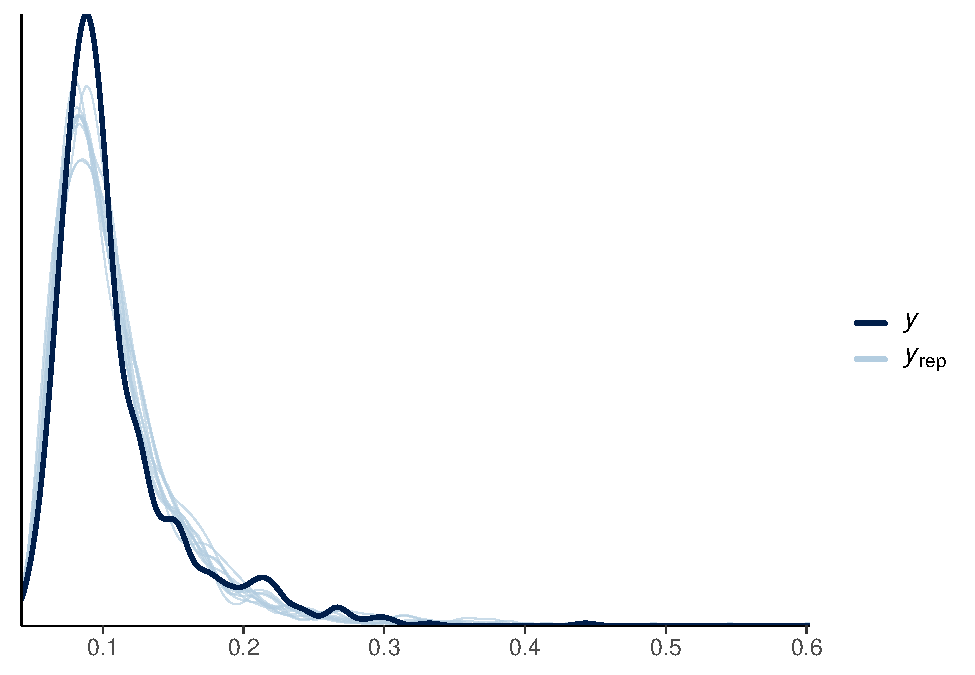
\includegraphics{params_analyses_files/figure-latex/unnamed-chunk-3-2.pdf}

\begin{Shaded}
\begin{Highlighting}[]
\FunctionTok{summary}\NormalTok{(m2)}
\end{Highlighting}
\end{Shaded}

\begin{verbatim}
## Warning: Parts of the model have not converged (some Rhats are > 1.05). Be
## careful when analysing the results! We recommend running more iterations and/or
## setting stronger priors.
\end{verbatim}

\begin{verbatim}
## Warning: There were 81 divergent transitions after warmup. Increasing
## adapt_delta above 0.8 may help. See
## http://mc-stan.org/misc/warnings.html#divergent-transitions-after-warmup
\end{verbatim}

\begin{verbatim}
##  Family: shifted_lognormal 
##   Links: mu = identity; sigma = identity; ndt = identity 
## Formula: C ~ exp * blk + (1 + blk | subject) 
##    Data: df (Number of observations: 736) 
##   Draws: 4 chains, each with iter = 2000; warmup = 1000; thin = 1;
##          total post-warmup draws = 4000
## 
## Group-Level Effects: 
## ~subject (Number of levels: 184) 
##                     Estimate Est.Error l-95% CI u-95% CI Rhat Bulk_ESS Tail_ESS
## sd(Intercept)           0.41      0.05     0.32     0.51 1.08       37      288
## sd(blk2)                0.15      0.10     0.01     0.35 1.10       31      124
## sd(blk3)                0.20      0.12     0.01     0.40 1.12       26      273
## sd(blk4)                0.22      0.11     0.02     0.42 1.11       26       84
## cor(Intercept,blk2)    -0.35      0.32    -0.79     0.50 1.03      210     1024
## cor(Intercept,blk3)    -0.34      0.29    -0.73     0.44 1.03      203      735
## cor(blk2,blk3)          0.39      0.41    -0.64     0.90 1.05      100      734
## cor(Intercept,blk4)    -0.62      0.20    -0.88    -0.08 1.03     1201      482
## cor(blk2,blk4)          0.54      0.40    -0.51     0.95 1.07       50      859
## cor(blk3,blk4)          0.59      0.38    -0.48     0.95 1.04       92      566
## 
## Population-Level Effects: 
##                  Estimate Est.Error l-95% CI u-95% CI Rhat Bulk_ESS Tail_ESS
## Intercept           -2.67      0.07    -2.81    -2.53 1.00     1072     1672
## expsurprise          0.32      0.08     0.17     0.47 1.00      897     1554
## blk2                -0.14      0.06    -0.25    -0.03 1.00      596     2114
## blk3                -0.15      0.06    -0.27    -0.03 1.00      810     1250
## blk4                -0.17      0.06    -0.29    -0.06 1.00      852     1488
## expsurprise:blk2    -0.13      0.07    -0.28     0.01 1.00     1015     1778
## expsurprise:blk3    -0.21      0.08    -0.36    -0.06 1.00      885     1033
## expsurprise:blk4    -0.24      0.08    -0.39    -0.09 1.00     1027     1454
## 
## Family Specific Parameters: 
##       Estimate Est.Error l-95% CI u-95% CI Rhat Bulk_ESS Tail_ESS
## sigma     0.32      0.03     0.25     0.37 1.09       36      209
## ndt       0.03      0.00     0.02     0.03 1.00     1013     1886
## 
## Draws were sampled using sample(hmc). For each parameter, Bulk_ESS
## and Tail_ESS are effective sample size measures, and Rhat is the potential
## scale reduction factor on split chains (at convergence, Rhat = 1).
\end{verbatim}

\begin{Shaded}
\begin{Highlighting}[]
\FunctionTok{conditional\_effects}\NormalTok{(m2, }\StringTok{"blk:exp"}\NormalTok{)}
\end{Highlighting}
\end{Shaded}

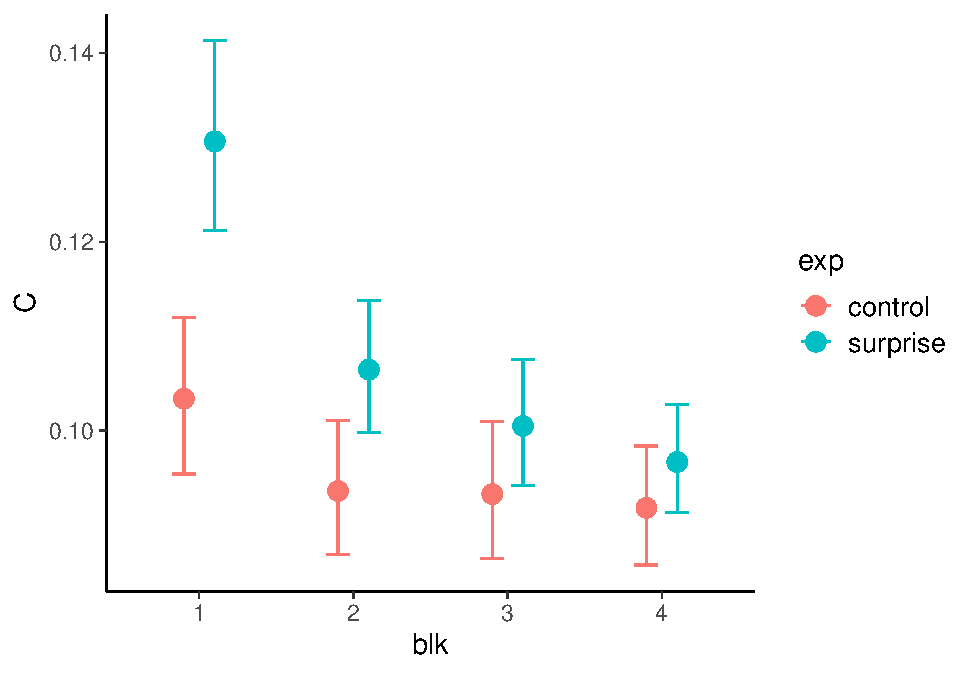
\includegraphics{params_analyses_files/figure-latex/unnamed-chunk-3-3.pdf}

Parameter mu\_ta: Drift rate for central target during response
selection phase 1

\begin{Shaded}
\begin{Highlighting}[]
\FunctionTok{plot}\NormalTok{(}\FunctionTok{density}\NormalTok{(df}\SpecialCharTok{$}\NormalTok{mu\_ta))}
\end{Highlighting}
\end{Shaded}

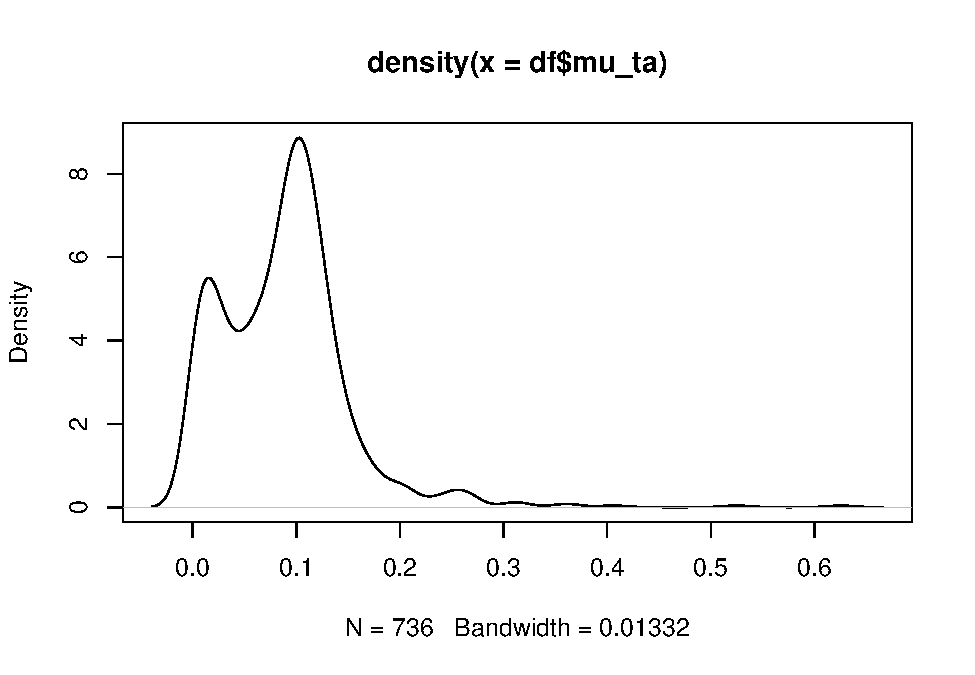
\includegraphics{params_analyses_files/figure-latex/unnamed-chunk-4-1.pdf}

\begin{Shaded}
\begin{Highlighting}[]
\NormalTok{m3 }\OtherTok{\textless{}{-}} \FunctionTok{brm}\NormalTok{(}
\NormalTok{  mu\_ta }\SpecialCharTok{\textasciitilde{}}\NormalTok{ exp }\SpecialCharTok{*}\NormalTok{ blk }\SpecialCharTok{+}\NormalTok{ (}\DecValTok{1} \SpecialCharTok{+}\NormalTok{ blk }\SpecialCharTok{|}\NormalTok{ subject),}
  \AttributeTok{family =} \FunctionTok{student}\NormalTok{(),}
  \AttributeTok{backend =} \StringTok{"cmdstanr"}\NormalTok{,}
  \CommentTok{\# algorithm = "meanfield",}
  \AttributeTok{data =}\NormalTok{ df}
\NormalTok{)}
\end{Highlighting}
\end{Shaded}

\begin{verbatim}
## In file included from /var/folders/cl/wwjrsxdd5tz7y9jr82nd5hrw0000gn/T/RtmpDVAVEa/model-d440365afac4.hpp:1:
## In file included from /Users/corrado/.cmdstan/cmdstan-2.33.1/stan/src/stan/model/model_header.hpp:4:
## In file included from /Users/corrado/.cmdstan/cmdstan-2.33.1/stan/lib/stan_math/stan/math.hpp:19:
## In file included from /Users/corrado/.cmdstan/cmdstan-2.33.1/stan/lib/stan_math/stan/math/rev.hpp:10:
## In file included from /Users/corrado/.cmdstan/cmdstan-2.33.1/stan/lib/stan_math/stan/math/rev/fun.hpp:200:
## In file included from /Users/corrado/.cmdstan/cmdstan-2.33.1/stan/lib/stan_math/stan/math/prim/functor.hpp:16:
## In file included from /Users/corrado/.cmdstan/cmdstan-2.33.1/stan/lib/stan_math/stan/math/prim/functor/integrate_ode_rk45.hpp:6:
## In file included from /Users/corrado/.cmdstan/cmdstan-2.33.1/stan/lib/stan_math/stan/math/prim/functor/ode_rk45.hpp:9:
## In file included from /Users/corrado/.cmdstan/cmdstan-2.33.1/stan/lib/stan_math/lib/boost_1.78.0/boost/numeric/odeint.hpp:76:
## In file included from /Users/corrado/.cmdstan/cmdstan-2.33.1/stan/lib/stan_math/lib/boost_1.78.0/boost/numeric/odeint/integrate/observer_collection.hpp:23:
## In file included from /Users/corrado/.cmdstan/cmdstan-2.33.1/stan/lib/stan_math/lib/boost_1.78.0/boost/function.hpp:30:
## In file included from /Users/corrado/.cmdstan/cmdstan-2.33.1/stan/lib/stan_math/lib/boost_1.78.0/boost/function/detail/prologue.hpp:17:
## In file included from /Users/corrado/.cmdstan/cmdstan-2.33.1/stan/lib/stan_math/lib/boost_1.78.0/boost/function/function_base.hpp:21:
## In file included from /Users/corrado/.cmdstan/cmdstan-2.33.1/stan/lib/stan_math/lib/boost_1.78.0/boost/type_index.hpp:29:
## In file included from /Users/corrado/.cmdstan/cmdstan-2.33.1/stan/lib/stan_math/lib/boost_1.78.0/boost/type_index/stl_type_index.hpp:47:
## /Users/corrado/.cmdstan/cmdstan-2.33.1/stan/lib/stan_math/lib/boost_1.78.0/boost/container_hash/hash.hpp:132:33: warning: 'unary_function<const std::error_category *, unsigned long>' is deprecat
\end{verbatim}

\begin{verbatim}
## ed [-Wdeprecated-declarations]
##         struct hash_base : std::unary_function<T, std::size_t> {};
##                                 ^
## /Users/corrado/.cmdstan/cmdstan-2.33.1/stan/lib/stan_math/lib/boost_1.78.0/boost/container_hash/hash.hpp:692:18: note: in instantiation of template class 'boost::hash_detail::hash_base<const std::error_category *>' requested here
##         : public boost::hash_detail::hash_base<T*>
##                  ^
## /Users/corrado/.cmdstan/cmdstan-2.33.1/stan/lib/stan_math/lib/boost_1.78.0/boost/container_hash/hash.hpp:420:24: note: in instantiation of template class 'boost::hash<const std::error_category *>' requested here
##         boost::hash<T> hasher;
##                        ^
## /Users/corrado/.cmdstan/cmdstan-2.33.1/stan/lib/stan_math/lib/boost_1.78.0/boost/container_hash/hash.hpp:551:9: note: in instantiation of function template specialization 'boost::hash_combine<const std::error_category *>' requested here
##         hash_combine(seed, &v.category());
##         ^
\end{verbatim}

\begin{verbatim}
## /Library/Developer/CommandLineTools/SDKs/MacOSX.sdk/usr/include/c++/v1/__functional/unary_function.h:23:29: note: 'unary_function<const std::error_category *, unsigned long>' has been explicitly marked deprecated here
## struct _LIBCPP_TEMPLATE_VIS _LIBCPP_DEPRECATED_IN_CXX11 unary_function
##                             ^
## /Library/Developer/CommandLineTools/SDKs/MacOSX.sdk/usr/include/c++/v1/__config:825:41: note: expanded from macro '_LIBCPP_DEPRECATED_IN_CXX11'
## #    define _LIBCPP_DEPRECATED_IN_CXX11 _LIBCPP_DEPRECATED
##                                         ^
## /Library/Developer/CommandLineTools/SDKs/MacOSX.sdk/usr/include/c++/v1/__config:810:49: note: expanded from macro '_LIBCPP_DEPRECATED'
## #      define _LIBCPP_DEPRECATED __attribute__((deprecated))
##                                                 ^
\end{verbatim}

\begin{verbatim}
## 1 warning generated.
\end{verbatim}

\begin{verbatim}
## Start sampling
\end{verbatim}

\begin{verbatim}
## Running MCMC with 4 sequential chains...
## 
## Chain 1 Iteration:    1 / 2000 [  0%]  (Warmup) 
## Chain 1 Iteration:  100 / 2000 [  5%]  (Warmup) 
## Chain 1 Iteration:  200 / 2000 [ 10%]  (Warmup) 
## Chain 1 Iteration:  300 / 2000 [ 15%]  (Warmup) 
## Chain 1 Iteration:  400 / 2000 [ 20%]  (Warmup) 
## Chain 1 Iteration:  500 / 2000 [ 25%]  (Warmup) 
## Chain 1 Iteration:  600 / 2000 [ 30%]  (Warmup) 
## Chain 1 Iteration:  700 / 2000 [ 35%]  (Warmup) 
## Chain 1 Iteration:  800 / 2000 [ 40%]  (Warmup) 
## Chain 1 Iteration:  900 / 2000 [ 45%]  (Warmup) 
## Chain 1 Iteration: 1000 / 2000 [ 50%]  (Warmup) 
## Chain 1 Iteration: 1001 / 2000 [ 50%]  (Sampling) 
## Chain 1 Iteration: 1100 / 2000 [ 55%]  (Sampling) 
## Chain 1 Iteration: 1200 / 2000 [ 60%]  (Sampling) 
## Chain 1 Iteration: 1300 / 2000 [ 65%]  (Sampling) 
## Chain 1 Iteration: 1400 / 2000 [ 70%]  (Sampling) 
## Chain 1 Iteration: 1500 / 2000 [ 75%]  (Sampling) 
## Chain 1 Iteration: 1600 / 2000 [ 80%]  (Sampling) 
## Chain 1 Iteration: 1700 / 2000 [ 85%]  (Sampling) 
## Chain 1 Iteration: 1800 / 2000 [ 90%]  (Sampling) 
## Chain 1 Iteration: 1900 / 2000 [ 95%]  (Sampling) 
## Chain 1 Iteration: 2000 / 2000 [100%]  (Sampling) 
## Chain 1 finished in 11.4 seconds.
## Chain 2 Iteration:    1 / 2000 [  0%]  (Warmup) 
## Chain 2 Iteration:  100 / 2000 [  5%]  (Warmup) 
## Chain 2 Iteration:  200 / 2000 [ 10%]  (Warmup) 
## Chain 2 Iteration:  300 / 2000 [ 15%]  (Warmup) 
## Chain 2 Iteration:  400 / 2000 [ 20%]  (Warmup) 
## Chain 2 Iteration:  500 / 2000 [ 25%]  (Warmup) 
## Chain 2 Iteration:  600 / 2000 [ 30%]  (Warmup) 
## Chain 2 Iteration:  700 / 2000 [ 35%]  (Warmup) 
## Chain 2 Iteration:  800 / 2000 [ 40%]  (Warmup) 
## Chain 2 Iteration:  900 / 2000 [ 45%]  (Warmup) 
## Chain 2 Iteration: 1000 / 2000 [ 50%]  (Warmup) 
## Chain 2 Iteration: 1001 / 2000 [ 50%]  (Sampling) 
## Chain 2 Iteration: 1100 / 2000 [ 55%]  (Sampling) 
## Chain 2 Iteration: 1200 / 2000 [ 60%]  (Sampling) 
## Chain 2 Iteration: 1300 / 2000 [ 65%]  (Sampling) 
## Chain 2 Iteration: 1400 / 2000 [ 70%]  (Sampling) 
## Chain 2 Iteration: 1500 / 2000 [ 75%]  (Sampling) 
## Chain 2 Iteration: 1600 / 2000 [ 80%]  (Sampling) 
## Chain 2 Iteration: 1700 / 2000 [ 85%]  (Sampling) 
## Chain 2 Iteration: 1800 / 2000 [ 90%]  (Sampling) 
## Chain 2 Iteration: 1900 / 2000 [ 95%]  (Sampling) 
## Chain 2 Iteration: 2000 / 2000 [100%]  (Sampling) 
## Chain 2 finished in 13.0 seconds.
## Chain 3 Iteration:    1 / 2000 [  0%]  (Warmup) 
## Chain 3 Iteration:  100 / 2000 [  5%]  (Warmup) 
## Chain 3 Iteration:  200 / 2000 [ 10%]  (Warmup) 
## Chain 3 Iteration:  300 / 2000 [ 15%]  (Warmup) 
## Chain 3 Iteration:  400 / 2000 [ 20%]  (Warmup) 
## Chain 3 Iteration:  500 / 2000 [ 25%]  (Warmup) 
## Chain 3 Iteration:  600 / 2000 [ 30%]  (Warmup) 
## Chain 3 Iteration:  700 / 2000 [ 35%]  (Warmup) 
## Chain 3 Iteration:  800 / 2000 [ 40%]  (Warmup) 
## Chain 3 Iteration:  900 / 2000 [ 45%]  (Warmup) 
## Chain 3 Iteration: 1000 / 2000 [ 50%]  (Warmup) 
## Chain 3 Iteration: 1001 / 2000 [ 50%]  (Sampling) 
## Chain 3 Iteration: 1100 / 2000 [ 55%]  (Sampling) 
## Chain 3 Iteration: 1200 / 2000 [ 60%]  (Sampling) 
## Chain 3 Iteration: 1300 / 2000 [ 65%]  (Sampling) 
## Chain 3 Iteration: 1400 / 2000 [ 70%]  (Sampling) 
## Chain 3 Iteration: 1500 / 2000 [ 75%]  (Sampling) 
## Chain 3 Iteration: 1600 / 2000 [ 80%]  (Sampling) 
## Chain 3 Iteration: 1700 / 2000 [ 85%]  (Sampling) 
## Chain 3 Iteration: 1800 / 2000 [ 90%]  (Sampling) 
## Chain 3 Iteration: 1900 / 2000 [ 95%]  (Sampling) 
## Chain 3 Iteration: 2000 / 2000 [100%]  (Sampling) 
## Chain 3 finished in 11.0 seconds.
## Chain 4 Iteration:    1 / 2000 [  0%]  (Warmup) 
## Chain 4 Iteration:  100 / 2000 [  5%]  (Warmup) 
## Chain 4 Iteration:  200 / 2000 [ 10%]  (Warmup) 
## Chain 4 Iteration:  300 / 2000 [ 15%]  (Warmup) 
## Chain 4 Iteration:  400 / 2000 [ 20%]  (Warmup) 
## Chain 4 Iteration:  500 / 2000 [ 25%]  (Warmup) 
## Chain 4 Iteration:  600 / 2000 [ 30%]  (Warmup) 
## Chain 4 Iteration:  700 / 2000 [ 35%]  (Warmup) 
## Chain 4 Iteration:  800 / 2000 [ 40%]  (Warmup) 
## Chain 4 Iteration:  900 / 2000 [ 45%]  (Warmup) 
## Chain 4 Iteration: 1000 / 2000 [ 50%]  (Warmup) 
## Chain 4 Iteration: 1001 / 2000 [ 50%]  (Sampling) 
## Chain 4 Iteration: 1100 / 2000 [ 55%]  (Sampling) 
## Chain 4 Iteration: 1200 / 2000 [ 60%]  (Sampling) 
## Chain 4 Iteration: 1300 / 2000 [ 65%]  (Sampling) 
## Chain 4 Iteration: 1400 / 2000 [ 70%]  (Sampling) 
## Chain 4 Iteration: 1500 / 2000 [ 75%]  (Sampling) 
## Chain 4 Iteration: 1600 / 2000 [ 80%]  (Sampling) 
## Chain 4 Iteration: 1700 / 2000 [ 85%]  (Sampling) 
## Chain 4 Iteration: 1800 / 2000 [ 90%]  (Sampling) 
## Chain 4 Iteration: 1900 / 2000 [ 95%]  (Sampling) 
## Chain 4 Iteration: 2000 / 2000 [100%]  (Sampling) 
## Chain 4 finished in 12.4 seconds.
## 
## All 4 chains finished successfully.
## Mean chain execution time: 11.9 seconds.
## Total execution time: 48.1 seconds.
\end{verbatim}

\begin{verbatim}
## Warning: 1 of 4000 (0.0%) transitions ended with a divergence.
## See https://mc-stan.org/misc/warnings for details.
\end{verbatim}

\begin{Shaded}
\begin{Highlighting}[]
\FunctionTok{pp\_check}\NormalTok{(m3)}
\end{Highlighting}
\end{Shaded}

\begin{verbatim}
## Using 10 posterior draws for ppc type 'dens_overlay' by default.
\end{verbatim}

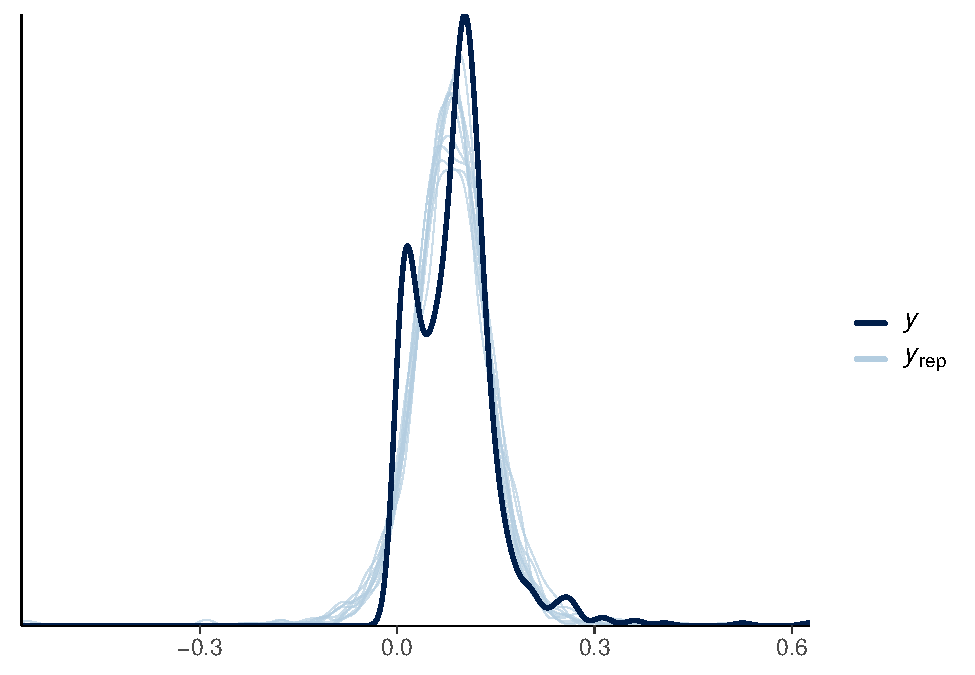
\includegraphics{params_analyses_files/figure-latex/unnamed-chunk-4-2.pdf}

\begin{Shaded}
\begin{Highlighting}[]
\FunctionTok{summary}\NormalTok{(m3)}
\end{Highlighting}
\end{Shaded}

\begin{verbatim}
## Warning: Parts of the model have not converged (some Rhats are > 1.05). Be
## careful when analysing the results! We recommend running more iterations and/or
## setting stronger priors.
\end{verbatim}

\begin{verbatim}
## Warning: There were 1 divergent transitions after warmup. Increasing
## adapt_delta above 0.8 may help. See
## http://mc-stan.org/misc/warnings.html#divergent-transitions-after-warmup
\end{verbatim}

\begin{verbatim}
##  Family: student 
##   Links: mu = identity; sigma = identity; nu = identity 
## Formula: mu_ta ~ exp * blk + (1 + blk | subject) 
##    Data: df (Number of observations: 736) 
##   Draws: 4 chains, each with iter = 2000; warmup = 1000; thin = 1;
##          total post-warmup draws = 4000
## 
## Group-Level Effects: 
## ~subject (Number of levels: 184) 
##                     Estimate Est.Error l-95% CI u-95% CI Rhat Bulk_ESS Tail_ESS
## sd(Intercept)           0.03      0.00     0.02     0.03 1.02      370      559
## sd(blk2)                0.01      0.01     0.00     0.03 1.01      383      387
## sd(blk3)                0.03      0.01     0.00     0.04 1.07       51      283
## sd(blk4)                0.04      0.01     0.02     0.05 1.06       66      237
## cor(Intercept,blk2)     0.03      0.40    -0.70     0.78 1.00     2524     2911
## cor(Intercept,blk3)    -0.18      0.29    -0.61     0.56 1.03      209      810
## cor(blk2,blk3)          0.21      0.42    -0.70     0.87 1.03      286      818
## cor(Intercept,blk4)    -0.33      0.21    -0.64     0.19 1.03      151      578
## cor(blk2,blk4)          0.11      0.40    -0.72     0.79 1.02      238      469
## cor(blk3,blk4)          0.56      0.27    -0.18     0.92 1.02      460      431
## 
## Population-Level Effects: 
##                  Estimate Est.Error l-95% CI u-95% CI Rhat Bulk_ESS Tail_ESS
## Intercept            0.07      0.01     0.06     0.09 1.00     1775     1699
## expsurprise          0.00      0.01    -0.01     0.02 1.00     1501     1228
## blk2                 0.01      0.01    -0.00     0.03 1.00     2569     3133
## blk3                 0.01      0.01    -0.01     0.03 1.00     1525     1683
## blk4                 0.02      0.01     0.00     0.03 1.00     1913     2841
## expsurprise:blk2    -0.01      0.01    -0.02     0.01 1.00     2339     2846
## expsurprise:blk3     0.00      0.01    -0.01     0.02 1.00     1427     1466
## expsurprise:blk4    -0.01      0.01    -0.04     0.01 1.00     1661     2601
## 
## Family Specific Parameters: 
##       Estimate Est.Error l-95% CI u-95% CI Rhat Bulk_ESS Tail_ESS
## sigma     0.03      0.00     0.03     0.04 1.05      101      275
## nu        3.23      0.58     2.28     4.50 1.02      267      615
## 
## Draws were sampled using sample(hmc). For each parameter, Bulk_ESS
## and Tail_ESS are effective sample size measures, and Rhat is the potential
## scale reduction factor on split chains (at convergence, Rhat = 1).
\end{verbatim}

\begin{Shaded}
\begin{Highlighting}[]
\FunctionTok{conditional\_effects}\NormalTok{(m3, }\StringTok{"blk:exp"}\NormalTok{)}
\end{Highlighting}
\end{Shaded}

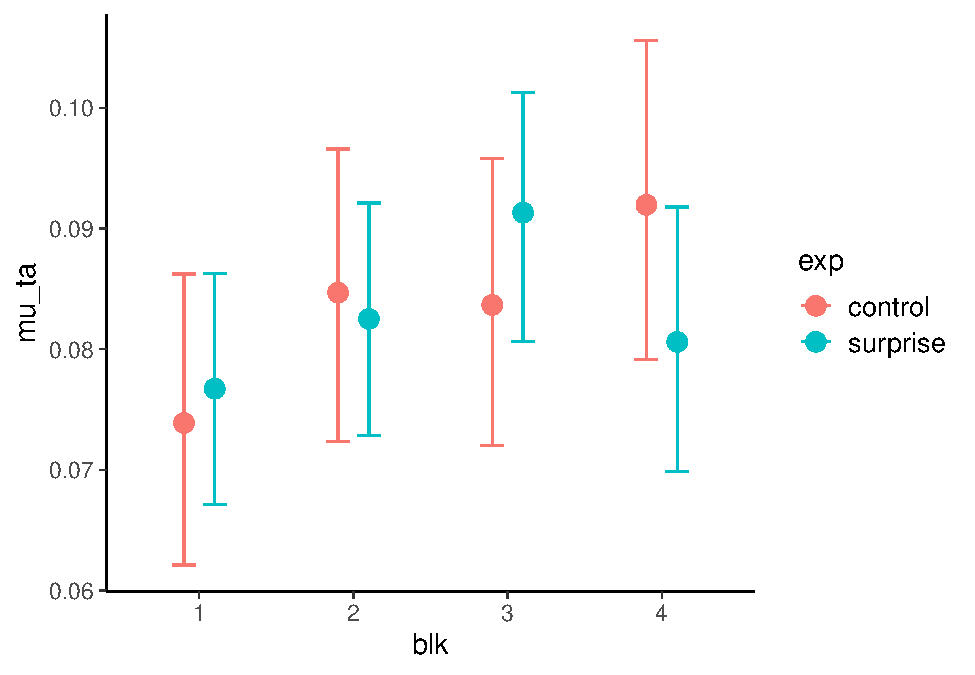
\includegraphics{params_analyses_files/figure-latex/unnamed-chunk-4-3.pdf}

Parameter mu\_fl: Drift rate for the flankers during response selection
phase 1

\begin{Shaded}
\begin{Highlighting}[]
\NormalTok{df }\SpecialCharTok{|\textgreater{}} 
  \FunctionTok{group\_by}\NormalTok{(exp, blk) }\SpecialCharTok{|\textgreater{}} 
  \FunctionTok{summarize}\NormalTok{(}
    \AttributeTok{mu\_fl =} \FunctionTok{mean}\NormalTok{(mu\_fl, }\AttributeTok{trim =} \FloatTok{0.1}\NormalTok{),}
    \AttributeTok{n =} \FunctionTok{n}\NormalTok{(),}
    \AttributeTok{stderr =} \FunctionTok{sqrt}\NormalTok{(}\FunctionTok{var}\NormalTok{(mu\_fl) }\SpecialCharTok{/}\NormalTok{ n)}
\NormalTok{  )}
\end{Highlighting}
\end{Shaded}

\begin{verbatim}
## `summarise()` has grouped output by 'exp'. You can override using the `.groups`
## argument.
\end{verbatim}

\begin{verbatim}
## # A tibble: 8 x 5
## # Groups:   exp [2]
##   exp      blk    mu_fl     n stderr
##   <chr>    <fct>  <dbl> <int>  <dbl>
## 1 control  1     0.0775    75     NA
## 2 control  2     0.0892    75     NA
## 3 control  3     0.103     75     NA
## 4 control  4     0.119     75     NA
## 5 surprise 1     0.0423   109     NA
## 6 surprise 2     0.0661   109     NA
## 7 surprise 3     0.0707   109     NA
## 8 surprise 4     0.0887   109     NA
\end{verbatim}

\begin{Shaded}
\begin{Highlighting}[]
\CommentTok{\# df$mu\_fl \textless{}{-} 0.001 + df$mu\_fl * 10}
\FunctionTok{plot}\NormalTok{(}\FunctionTok{density}\NormalTok{(df}\SpecialCharTok{$}\NormalTok{mu\_fl))}
\end{Highlighting}
\end{Shaded}

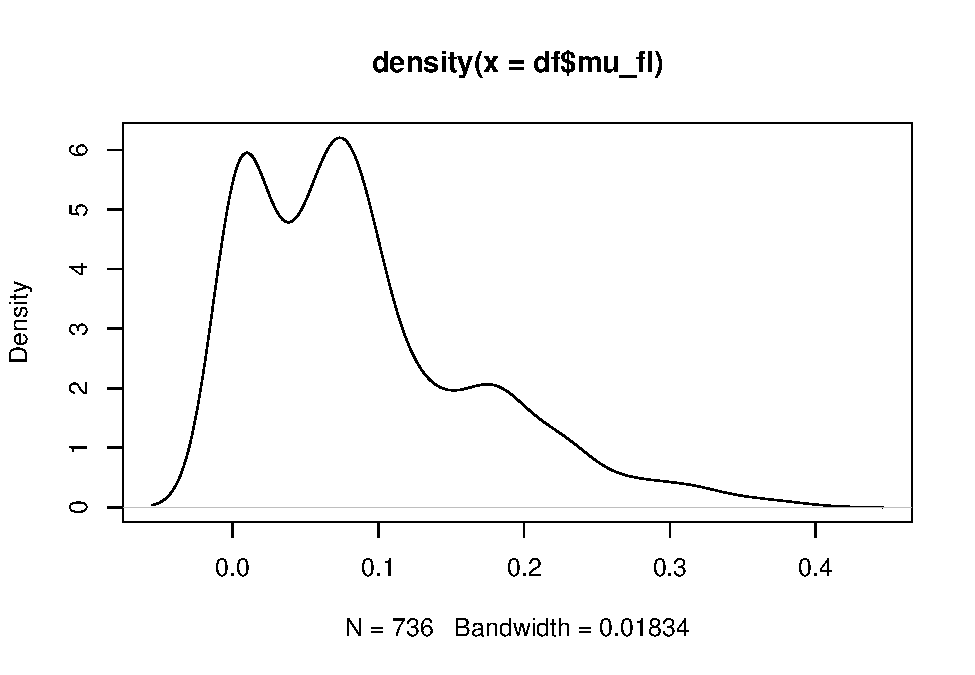
\includegraphics{params_analyses_files/figure-latex/unnamed-chunk-5-1.pdf}

\begin{Shaded}
\begin{Highlighting}[]
\NormalTok{m4 }\OtherTok{\textless{}{-}} \FunctionTok{brm}\NormalTok{(}
\NormalTok{  mu\_fl }\SpecialCharTok{\textasciitilde{}}\NormalTok{ exp }\SpecialCharTok{*}\NormalTok{ blk }\SpecialCharTok{+}\NormalTok{ (}\DecValTok{1} \SpecialCharTok{+}\NormalTok{ blk }\SpecialCharTok{|}\NormalTok{ subject),}
  \AttributeTok{family =} \FunctionTok{zero\_inflated\_beta}\NormalTok{(),}
  \AttributeTok{backend =} \StringTok{"cmdstanr"}\NormalTok{,}
  \CommentTok{\# control = list(max\_treedepth = 15, adapt\_delta = 0.95),}
  \CommentTok{\# algorithm = "meanfield",}
  \CommentTok{\# iter = 10000,}
  \AttributeTok{data =}\NormalTok{ df}
\NormalTok{)}
\end{Highlighting}
\end{Shaded}

\begin{verbatim}
## In file included from /var/folders/cl/wwjrsxdd5tz7y9jr82nd5hrw0000gn/T/RtmpDVAVEa/model-d44052c839e9.hpp:1:
## In file included from /Users/corrado/.cmdstan/cmdstan-2.33.1/stan/src/stan/model/model_header.hpp:4:
## In file included from /Users/corrado/.cmdstan/cmdstan-2.33.1/stan/lib/stan_math/stan/math.hpp:19:
## In file included from /Users/corrado/.cmdstan/cmdstan-2.33.1/stan/lib/stan_math/stan/math/rev.hpp:10:
## In file included from /Users/corrado/.cmdstan/cmdstan-2.33.1/stan/lib/stan_math/stan/math/rev/fun.hpp:200:
## In file included from /Users/corrado/.cmdstan/cmdstan-2.33.1/stan/lib/stan_math/stan/math/prim/functor.hpp:16:
## In file included from /Users/corrado/.cmdstan/cmdstan-2.33.1/stan/lib/stan_math/stan/math/prim/functor/integrate_ode_rk45.hpp:6:
## In file included from /Users/corrado/.cmdstan/cmdstan-2.33.1/stan/lib/stan_math/stan/math/prim/functor/ode_rk45.hpp:9:
## In file included from /Users/corrado/.cmdstan/cmdstan-2.33.1/stan/lib/stan_math/lib/boost_1.78.0/boost/numeric/odeint.hpp:76:
## In file included from /Users/corrado/.cmdstan/cmdstan-2.33.1/stan/lib/stan_math/lib/boost_1.78.0/boost/numeric/odeint/integrate/observer_collection.hpp:23:
## In file included from /Users/corrado/.cmdstan/cmdstan-2.33.1/stan/lib/stan_math/lib/boost_1.78.0/boost/function.hpp:30:
## In file included from /Users/corrado/.cmdstan/cmdstan-2.33.1/stan/lib/stan_math/lib/boost_1.78.0/boost/function/detail/prologue.hpp:17:
## In file included from /Users/corrado/.cmdstan/cmdstan-2.33.1/stan/lib/stan_math/lib/boost_1.78.0/boost/function/function_base.hpp:21:
## In file included from /Users/corrado/.cmdstan/cmdstan-2.33.1/stan/lib/stan_math/lib/boost_1.78.0/boost/type_index.hpp:29:
## In file included from /Users/corrado/.cmdstan/cmdstan-2.33.1/stan/lib/stan_math/lib/boost_1.78.0/boost/type_index/stl_type_index.hpp:47:
## /Users/corrado/.cmdstan/cmdstan-2.33.1/stan/lib/stan_math/lib/boost_1.78.0/boost/container_hash/hash.hpp:132:33: warning: 'unary_function<const std::error_category *, unsigned long>' is deprecat
## ed [-Wdeprecated-declarations]
##         struct hash_base : std::unary_function<T, std::size_t> {};
##                                 ^
## /Users/corrado/.cmdstan/cmdstan-2.33.1/stan/lib/stan_math/lib/boost_1.78.0/boost/container_hash/hash.hpp:692:18: note: in instantiation of template class 'boost::hash_detail::hash_base<const std::error_category *>' requested here
##         : public boost::hash_detail::hash_base<T*>
##                  ^
## /Users/corrado/.cmdstan/cmdstan-2.33.1/stan/lib/stan_math/lib/boost_1.78.0/boost/container_hash/hash.hpp:420:24: note: in instantiation of template class 'boost::hash<const std::error_category *>' requested here
##         boost::hash<T> hasher;
##                        ^
## /Users/corrado/.cmdstan/cmdstan-2.33.1/stan/lib/stan_math/lib/boost_1.78.0/boost/container_hash/hash.hpp:551:9: note: in instantiation of function template specialization 'boost::hash_combine<const std::error_category *>' requested here
##         hash_combine(seed, &v.category());
##         ^
## 
## /Library/Developer/CommandLineTools/SDKs/MacOSX.sdk/usr/include/c++/v1/__functional/unary_function.h:23:29: note: 'unary_function<const std::error_category *, unsigned long>' has been explicitly marked deprecated here
## struct _LIBCPP_TEMPLATE_VIS _LIBCPP_DEPRECATED_IN_CXX11 unary_function
##                             ^
## /Library/Developer/CommandLineTools/SDKs/MacOSX.sdk/usr/include/c++/v1/__config:825:41: note: expanded from macro '_LIBCPP_DEPRECATED_IN_CXX11'
## #    define _LIBCPP_DEPRECATED_IN_CXX11 _LIBCPP_DEPRECATED
##                                         ^
## /Library/Developer/CommandLineTools/SDKs/MacOSX.sdk/usr/include/c++/v1/__config:810:49: note: expanded from macro '_LIBCPP_DEPRECATED'
## #      define _LIBCPP_DEPRECATED __attribute__((deprecated))
##                                                 ^
## 
## 1 warning generated.
## 
## Start sampling
\end{verbatim}

\begin{verbatim}
## Running MCMC with 4 sequential chains...
## 
## Chain 1 Iteration:    1 / 2000 [  0%]  (Warmup) 
## Chain 1 Iteration:  100 / 2000 [  5%]  (Warmup) 
## Chain 1 Iteration:  200 / 2000 [ 10%]  (Warmup) 
## Chain 1 Iteration:  300 / 2000 [ 15%]  (Warmup) 
## Chain 1 Iteration:  400 / 2000 [ 20%]  (Warmup) 
## Chain 1 Iteration:  500 / 2000 [ 25%]  (Warmup) 
## Chain 1 Iteration:  600 / 2000 [ 30%]  (Warmup) 
## Chain 1 Iteration:  700 / 2000 [ 35%]  (Warmup) 
## Chain 1 Iteration:  800 / 2000 [ 40%]  (Warmup) 
## Chain 1 Iteration:  900 / 2000 [ 45%]  (Warmup) 
## Chain 1 Iteration: 1000 / 2000 [ 50%]  (Warmup) 
## Chain 1 Iteration: 1001 / 2000 [ 50%]  (Sampling) 
## Chain 1 Iteration: 1100 / 2000 [ 55%]  (Sampling) 
## Chain 1 Iteration: 1200 / 2000 [ 60%]  (Sampling) 
## Chain 1 Iteration: 1300 / 2000 [ 65%]  (Sampling) 
## Chain 1 Iteration: 1400 / 2000 [ 70%]  (Sampling) 
## Chain 1 Iteration: 1500 / 2000 [ 75%]  (Sampling) 
## Chain 1 Iteration: 1600 / 2000 [ 80%]  (Sampling) 
## Chain 1 Iteration: 1700 / 2000 [ 85%]  (Sampling) 
## Chain 1 Iteration: 1800 / 2000 [ 90%]  (Sampling) 
## Chain 1 Iteration: 1900 / 2000 [ 95%]  (Sampling) 
## Chain 1 Iteration: 2000 / 2000 [100%]  (Sampling) 
## Chain 1 finished in 20.0 seconds.
## Chain 2 Iteration:    1 / 2000 [  0%]  (Warmup) 
## Chain 2 Iteration:  100 / 2000 [  5%]  (Warmup) 
## Chain 2 Iteration:  200 / 2000 [ 10%]  (Warmup) 
## Chain 2 Iteration:  300 / 2000 [ 15%]  (Warmup) 
## Chain 2 Iteration:  400 / 2000 [ 20%]  (Warmup) 
## Chain 2 Iteration:  500 / 2000 [ 25%]  (Warmup) 
## Chain 2 Iteration:  600 / 2000 [ 30%]  (Warmup) 
## Chain 2 Iteration:  700 / 2000 [ 35%]  (Warmup) 
## Chain 2 Iteration:  800 / 2000 [ 40%]  (Warmup) 
## Chain 2 Iteration:  900 / 2000 [ 45%]  (Warmup) 
## Chain 2 Iteration: 1000 / 2000 [ 50%]  (Warmup) 
## Chain 2 Iteration: 1001 / 2000 [ 50%]  (Sampling) 
## Chain 2 Iteration: 1100 / 2000 [ 55%]  (Sampling) 
## Chain 2 Iteration: 1200 / 2000 [ 60%]  (Sampling) 
## Chain 2 Iteration: 1300 / 2000 [ 65%]  (Sampling) 
## Chain 2 Iteration: 1400 / 2000 [ 70%]  (Sampling) 
## Chain 2 Iteration: 1500 / 2000 [ 75%]  (Sampling) 
## Chain 2 Iteration: 1600 / 2000 [ 80%]  (Sampling) 
## Chain 2 Iteration: 1700 / 2000 [ 85%]  (Sampling) 
## Chain 2 Iteration: 1800 / 2000 [ 90%]  (Sampling) 
## Chain 2 Iteration: 1900 / 2000 [ 95%]  (Sampling) 
## Chain 2 Iteration: 2000 / 2000 [100%]  (Sampling) 
## Chain 2 finished in 20.0 seconds.
## Chain 3 Iteration:    1 / 2000 [  0%]  (Warmup) 
## Chain 3 Iteration:  100 / 2000 [  5%]  (Warmup) 
## Chain 3 Iteration:  200 / 2000 [ 10%]  (Warmup) 
## Chain 3 Iteration:  300 / 2000 [ 15%]  (Warmup) 
## Chain 3 Iteration:  400 / 2000 [ 20%]  (Warmup) 
## Chain 3 Iteration:  500 / 2000 [ 25%]  (Warmup) 
## Chain 3 Iteration:  600 / 2000 [ 30%]  (Warmup) 
## Chain 3 Iteration:  700 / 2000 [ 35%]  (Warmup) 
## Chain 3 Iteration:  800 / 2000 [ 40%]  (Warmup) 
## Chain 3 Iteration:  900 / 2000 [ 45%]  (Warmup) 
## Chain 3 Iteration: 1000 / 2000 [ 50%]  (Warmup) 
## Chain 3 Iteration: 1001 / 2000 [ 50%]  (Sampling) 
## Chain 3 Iteration: 1100 / 2000 [ 55%]  (Sampling) 
## Chain 3 Iteration: 1200 / 2000 [ 60%]  (Sampling) 
## Chain 3 Iteration: 1300 / 2000 [ 65%]  (Sampling) 
## Chain 3 Iteration: 1400 / 2000 [ 70%]  (Sampling) 
## Chain 3 Iteration: 1500 / 2000 [ 75%]  (Sampling) 
## Chain 3 Iteration: 1600 / 2000 [ 80%]  (Sampling) 
## Chain 3 Iteration: 1700 / 2000 [ 85%]  (Sampling) 
## Chain 3 Iteration: 1800 / 2000 [ 90%]  (Sampling) 
## Chain 3 Iteration: 1900 / 2000 [ 95%]  (Sampling) 
## Chain 3 Iteration: 2000 / 2000 [100%]  (Sampling) 
## Chain 3 finished in 18.9 seconds.
## Chain 4 Iteration:    1 / 2000 [  0%]  (Warmup) 
## Chain 4 Iteration:  100 / 2000 [  5%]  (Warmup) 
## Chain 4 Iteration:  200 / 2000 [ 10%]  (Warmup) 
## Chain 4 Iteration:  300 / 2000 [ 15%]  (Warmup) 
## Chain 4 Iteration:  400 / 2000 [ 20%]  (Warmup) 
## Chain 4 Iteration:  500 / 2000 [ 25%]  (Warmup) 
## Chain 4 Iteration:  600 / 2000 [ 30%]  (Warmup) 
## Chain 4 Iteration:  700 / 2000 [ 35%]  (Warmup) 
## Chain 4 Iteration:  800 / 2000 [ 40%]  (Warmup) 
## Chain 4 Iteration:  900 / 2000 [ 45%]  (Warmup) 
## Chain 4 Iteration: 1000 / 2000 [ 50%]  (Warmup) 
## Chain 4 Iteration: 1001 / 2000 [ 50%]  (Sampling) 
## Chain 4 Iteration: 1100 / 2000 [ 55%]  (Sampling) 
## Chain 4 Iteration: 1200 / 2000 [ 60%]  (Sampling) 
## Chain 4 Iteration: 1300 / 2000 [ 65%]  (Sampling) 
## Chain 4 Iteration: 1400 / 2000 [ 70%]  (Sampling) 
## Chain 4 Iteration: 1500 / 2000 [ 75%]  (Sampling) 
## Chain 4 Iteration: 1600 / 2000 [ 80%]  (Sampling) 
## Chain 4 Iteration: 1700 / 2000 [ 85%]  (Sampling) 
## Chain 4 Iteration: 1800 / 2000 [ 90%]  (Sampling) 
## Chain 4 Iteration: 1900 / 2000 [ 95%]  (Sampling) 
## Chain 4 Iteration: 2000 / 2000 [100%]  (Sampling) 
## Chain 4 finished in 19.8 seconds.
## 
## All 4 chains finished successfully.
## Mean chain execution time: 19.7 seconds.
## Total execution time: 79.0 seconds.
\end{verbatim}

\begin{verbatim}
## Warning: 2 of 4000 (0.0%) transitions ended with a divergence.
## See https://mc-stan.org/misc/warnings for details.
\end{verbatim}

\begin{Shaded}
\begin{Highlighting}[]
\FunctionTok{pp\_check}\NormalTok{(m4)}
\end{Highlighting}
\end{Shaded}

\begin{verbatim}
## Using 10 posterior draws for ppc type 'dens_overlay' by default.
\end{verbatim}

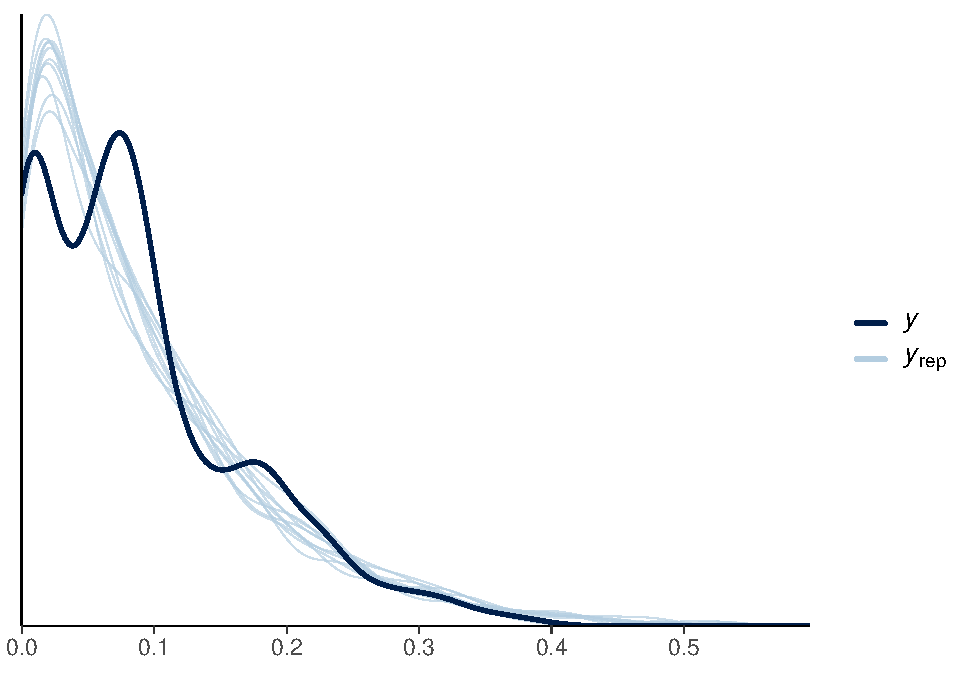
\includegraphics{params_analyses_files/figure-latex/unnamed-chunk-5-2.pdf}

\begin{Shaded}
\begin{Highlighting}[]
\FunctionTok{summary}\NormalTok{(m4)}
\end{Highlighting}
\end{Shaded}

\begin{verbatim}
## Warning: There were 2 divergent transitions after warmup. Increasing
## adapt_delta above 0.8 may help. See
## http://mc-stan.org/misc/warnings.html#divergent-transitions-after-warmup
\end{verbatim}

\begin{verbatim}
##  Family: zero_inflated_beta 
##   Links: mu = logit; phi = identity; zi = identity 
## Formula: mu_fl ~ exp * blk + (1 + blk | subject) 
##    Data: df (Number of observations: 736) 
##   Draws: 4 chains, each with iter = 2000; warmup = 1000; thin = 1;
##          total post-warmup draws = 4000
## 
## Group-Level Effects: 
## ~subject (Number of levels: 184) 
##                     Estimate Est.Error l-95% CI u-95% CI Rhat Bulk_ESS Tail_ESS
## sd(Intercept)           0.76      0.06     0.65     0.88 1.00     1258     1905
## sd(blk2)                0.13      0.10     0.00     0.35 1.01      657      737
## sd(blk3)                0.17      0.11     0.01     0.41 1.00      505      767
## sd(blk4)                0.12      0.09     0.00     0.34 1.01      546      505
## cor(Intercept,blk2)     0.11      0.38    -0.65     0.80 1.00     4322     2361
## cor(Intercept,blk3)     0.19      0.35    -0.58     0.81 1.00     3351     2491
## cor(blk2,blk3)          0.12      0.43    -0.75     0.85 1.00     1269     2099
## cor(Intercept,blk4)    -0.13      0.39    -0.80     0.68 1.00     3958     2208
## cor(blk2,blk4)          0.14      0.46    -0.76     0.88 1.01     1291     2129
## cor(blk3,blk4)          0.03      0.45    -0.79     0.81 1.00     2019     2861
## 
## Population-Level Effects: 
##                  Estimate Est.Error l-95% CI u-95% CI Rhat Bulk_ESS Tail_ESS
## Intercept           -2.59      0.12    -2.83    -2.35 1.00     1260     2052
## expsurprise         -0.53      0.16    -0.84    -0.22 1.00      987     1634
## blk2                 0.18      0.11    -0.04     0.41 1.00     2326     2487
## blk3                 0.31      0.12     0.09     0.54 1.00     2217     2424
## blk4                 0.49      0.11     0.28     0.71 1.00     2185     2282
## expsurprise:blk2     0.25      0.15    -0.05     0.54 1.00     2309     2467
## expsurprise:blk3     0.05      0.15    -0.25     0.35 1.00     2247     2538
## expsurprise:blk4     0.21      0.15    -0.09     0.49 1.00     2139     2327
## 
## Family Specific Parameters: 
##     Estimate Est.Error l-95% CI u-95% CI Rhat Bulk_ESS Tail_ESS
## phi    24.49      1.75    21.28    28.02 1.00     1187     1594
## zi      0.03      0.01     0.02     0.05 1.00     6723     2662
## 
## Draws were sampled using sample(hmc). For each parameter, Bulk_ESS
## and Tail_ESS are effective sample size measures, and Rhat is the potential
## scale reduction factor on split chains (at convergence, Rhat = 1).
\end{verbatim}

\begin{Shaded}
\begin{Highlighting}[]
\FunctionTok{conditional\_effects}\NormalTok{(m4, }\StringTok{"blk:exp"}\NormalTok{)}
\end{Highlighting}
\end{Shaded}

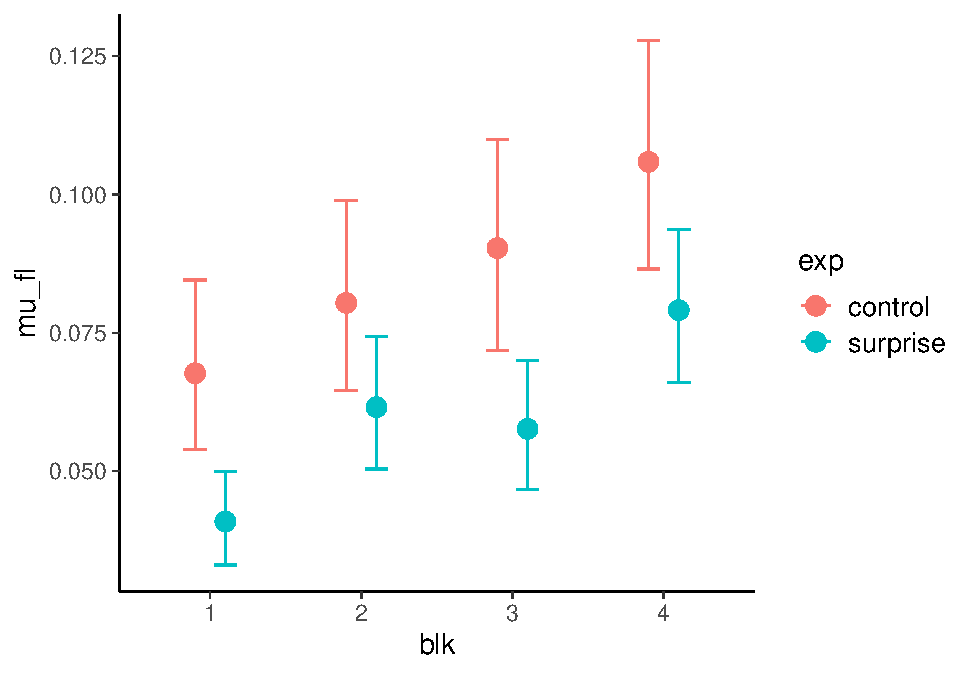
\includegraphics{params_analyses_files/figure-latex/unnamed-chunk-5-3.pdf}

Parameter mu\_ss: Drift rate for stimulus selection

\begin{Shaded}
\begin{Highlighting}[]
\FunctionTok{hist}\NormalTok{(df}\SpecialCharTok{$}\NormalTok{mu\_ss)}
\end{Highlighting}
\end{Shaded}

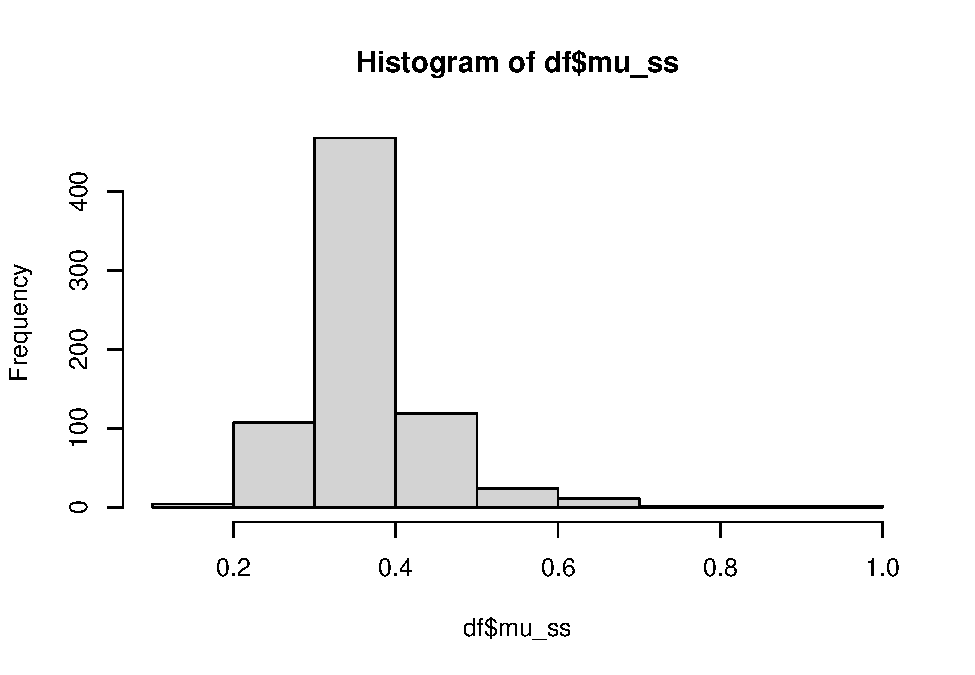
\includegraphics{params_analyses_files/figure-latex/unnamed-chunk-6-1.pdf}

\begin{Shaded}
\begin{Highlighting}[]
\NormalTok{m5 }\OtherTok{\textless{}{-}} \FunctionTok{brm}\NormalTok{(}
\NormalTok{  mu\_ss }\SpecialCharTok{\textasciitilde{}}\NormalTok{ exp }\SpecialCharTok{*}\NormalTok{ blk }\SpecialCharTok{+}\NormalTok{ (}\DecValTok{1} \SpecialCharTok{+}\NormalTok{ blk }\SpecialCharTok{|}\NormalTok{ subject),}
  \AttributeTok{family =} \FunctionTok{student}\NormalTok{(),}
  \AttributeTok{backend =} \StringTok{"cmdstanr"}\NormalTok{,}
  \CommentTok{\# algorithm = "meanfield",}
  \AttributeTok{data =}\NormalTok{ df}
\NormalTok{)}
\end{Highlighting}
\end{Shaded}

\begin{verbatim}
## In file included from /var/folders/cl/wwjrsxdd5tz7y9jr82nd5hrw0000gn/T/RtmpDVAVEa/model-d4405613fe24.hpp:1:
## In file included from /Users/corrado/.cmdstan/cmdstan-2.33.1/stan/src/stan/model/model_header.hpp:4:
## In file included from /Users/corrado/.cmdstan/cmdstan-2.33.1/stan/lib/stan_math/stan/math.hpp:19:
## In file included from /Users/corrado/.cmdstan/cmdstan-2.33.1/stan/lib/stan_math/stan/math/rev.hpp:10:
## In file included from /Users/corrado/.cmdstan/cmdstan-2.33.1/stan/lib/stan_math/stan/math/rev/fun.hpp:200:
## In file included from /Users/corrado/.cmdstan/cmdstan-2.33.1/stan/lib/stan_math/stan/math/prim/functor.hpp:16:
## In file included from /Users/corrado/.cmdstan/cmdstan-2.33.1/stan/lib/stan_math/stan/math/prim/functor/integrate_ode_rk45.hpp:6:
## In file included from /Users/corrado/.cmdstan/cmdstan-2.33.1/stan/lib/stan_math/stan/math/prim/functor/ode_rk45.hpp:9:
## In file included from /Users/corrado/.cmdstan/cmdstan-2.33.1/stan/lib/stan_math/lib/boost_1.78.0/boost/numeric/odeint.hpp:76:
## In file included from /Users/corrado/.cmdstan/cmdstan-2.33.1/stan/lib/stan_math/lib/boost_1.78.0/boost/numeric/odeint/integrate/observer_collection.hpp:23:
## In file included from /Users/corrado/.cmdstan/cmdstan-2.33.1/stan/lib/stan_math/lib/boost_1.78.0/boost/function.hpp:30:
## In file included from /Users/corrado/.cmdstan/cmdstan-2.33.1/stan/lib/stan_math/lib/boost_1.78.0/boost/function/detail/prologue.hpp:17:
## In file included from /Users/corrado/.cmdstan/cmdstan-2.33.1/stan/lib/stan_math/lib/boost_1.78.0/boost/function/function_base.hpp:21:
## In file included from /Users/corrado/.cmdstan/cmdstan-2.33.1/stan/lib/stan_math/lib/boost_1.78.0/boost/type_index.hpp:29:
## In file included from /Users/corrado/.cmdstan/cmdstan-2.33.1/stan/lib/stan_math/lib/boost_1.78.0/boost/type_index/stl_type_index.hpp:47:
## /Users/corrado/.cmdstan/cmdstan-2.33.1/stan/lib/stan_math/lib/boost_1.78.0/boost/container_hash/hash.hpp:132:33: warning: 'unary_function<const std::error_category *, unsigned long>' is deprecat
\end{verbatim}

\begin{verbatim}
## ed [-Wdeprecated-declarations]
##         struct hash_base : std::unary_function<T, std::size_t> {};
##                                 ^
## /Users/corrado/.cmdstan/cmdstan-2.33.1/stan/lib/stan_math/lib/boost_1.78.0/boost/container_hash/hash.hpp:692:18: note: in instantiation of template class 'boost::hash_detail::hash_base<const std::error_category *>' requested here
##         : public boost::hash_detail::hash_base<T*>
##                  ^
## /Users/corrado/.cmdstan/cmdstan-2.33.1/stan/lib/stan_math/lib/boost_1.78.0/boost/container_hash/hash.hpp:420:24: note: in instantiation of template class 'boost::hash<const std::error_category *>' requested here
##         boost::hash<T> hasher;
##                        ^
## /Users/corrado/.cmdstan/cmdstan-2.33.1/stan/lib/stan_math/lib/boost_1.78.0/boost/container_hash/hash.hpp:551:9: note: in instantiation of function template specialization 'boost::hash_combine<const std::error_category *>' requested here
##         hash_combine(seed, &v.category());
##         ^
\end{verbatim}

\begin{verbatim}
## /Library/Developer/CommandLineTools/SDKs/MacOSX.sdk/usr/include/c++/v1/__functional/unary_function.h:23:29: note: 'unary_function<const std::error_category *, unsigned long>' has been explicitly marked deprecated here
## struct _LIBCPP_TEMPLATE_VIS _LIBCPP_DEPRECATED_IN_CXX11 unary_function
##                             ^
## /Library/Developer/CommandLineTools/SDKs/MacOSX.sdk/usr/include/c++/v1/__config:825:41: note: expanded from macro '_LIBCPP_DEPRECATED_IN_CXX11'
## #    define _LIBCPP_DEPRECATED_IN_CXX11 _LIBCPP_DEPRECATED
##                                         ^
## /Library/Developer/CommandLineTools/SDKs/MacOSX.sdk/usr/include/c++/v1/__config:810:49: note: expanded from macro '_LIBCPP_DEPRECATED'
## #      define _LIBCPP_DEPRECATED __attribute__((deprecated))
##                                                 ^
\end{verbatim}

\begin{verbatim}
## 1 warning generated.
\end{verbatim}

\begin{verbatim}
## Start sampling
\end{verbatim}

\begin{verbatim}
## Running MCMC with 4 sequential chains...
## 
## Chain 1 Iteration:    1 / 2000 [  0%]  (Warmup) 
## Chain 1 Iteration:  100 / 2000 [  5%]  (Warmup) 
## Chain 1 Iteration:  200 / 2000 [ 10%]  (Warmup) 
## Chain 1 Iteration:  300 / 2000 [ 15%]  (Warmup) 
## Chain 1 Iteration:  400 / 2000 [ 20%]  (Warmup) 
## Chain 1 Iteration:  500 / 2000 [ 25%]  (Warmup) 
## Chain 1 Iteration:  600 / 2000 [ 30%]  (Warmup) 
## Chain 1 Iteration:  700 / 2000 [ 35%]  (Warmup) 
## Chain 1 Iteration:  800 / 2000 [ 40%]  (Warmup) 
## Chain 1 Iteration:  900 / 2000 [ 45%]  (Warmup) 
## Chain 1 Iteration: 1000 / 2000 [ 50%]  (Warmup) 
## Chain 1 Iteration: 1001 / 2000 [ 50%]  (Sampling) 
## Chain 1 Iteration: 1100 / 2000 [ 55%]  (Sampling) 
## Chain 1 Iteration: 1200 / 2000 [ 60%]  (Sampling) 
## Chain 1 Iteration: 1300 / 2000 [ 65%]  (Sampling) 
## Chain 1 Iteration: 1400 / 2000 [ 70%]  (Sampling) 
## Chain 1 Iteration: 1500 / 2000 [ 75%]  (Sampling) 
## Chain 1 Iteration: 1600 / 2000 [ 80%]  (Sampling) 
## Chain 1 Iteration: 1700 / 2000 [ 85%]  (Sampling) 
## Chain 1 Iteration: 1800 / 2000 [ 90%]  (Sampling) 
## Chain 1 Iteration: 1900 / 2000 [ 95%]  (Sampling) 
## Chain 1 Iteration: 2000 / 2000 [100%]  (Sampling) 
## Chain 1 finished in 11.2 seconds.
## Chain 2 Iteration:    1 / 2000 [  0%]  (Warmup) 
## Chain 2 Iteration:  100 / 2000 [  5%]  (Warmup) 
## Chain 2 Iteration:  200 / 2000 [ 10%]  (Warmup) 
## Chain 2 Iteration:  300 / 2000 [ 15%]  (Warmup) 
## Chain 2 Iteration:  400 / 2000 [ 20%]  (Warmup) 
## Chain 2 Iteration:  500 / 2000 [ 25%]  (Warmup) 
## Chain 2 Iteration:  600 / 2000 [ 30%]  (Warmup) 
## Chain 2 Iteration:  700 / 2000 [ 35%]  (Warmup) 
## Chain 2 Iteration:  800 / 2000 [ 40%]  (Warmup) 
## Chain 2 Iteration:  900 / 2000 [ 45%]  (Warmup) 
## Chain 2 Iteration: 1000 / 2000 [ 50%]  (Warmup) 
## Chain 2 Iteration: 1001 / 2000 [ 50%]  (Sampling) 
## Chain 2 Iteration: 1100 / 2000 [ 55%]  (Sampling) 
## Chain 2 Iteration: 1200 / 2000 [ 60%]  (Sampling) 
## Chain 2 Iteration: 1300 / 2000 [ 65%]  (Sampling) 
## Chain 2 Iteration: 1400 / 2000 [ 70%]  (Sampling) 
## Chain 2 Iteration: 1500 / 2000 [ 75%]  (Sampling) 
## Chain 2 Iteration: 1600 / 2000 [ 80%]  (Sampling) 
## Chain 2 Iteration: 1700 / 2000 [ 85%]  (Sampling) 
## Chain 2 Iteration: 1800 / 2000 [ 90%]  (Sampling) 
## Chain 2 Iteration: 1900 / 2000 [ 95%]  (Sampling) 
## Chain 2 Iteration: 2000 / 2000 [100%]  (Sampling) 
## Chain 2 finished in 11.1 seconds.
## Chain 3 Iteration:    1 / 2000 [  0%]  (Warmup) 
## Chain 3 Iteration:  100 / 2000 [  5%]  (Warmup) 
## Chain 3 Iteration:  200 / 2000 [ 10%]  (Warmup) 
## Chain 3 Iteration:  300 / 2000 [ 15%]  (Warmup) 
## Chain 3 Iteration:  400 / 2000 [ 20%]  (Warmup) 
## Chain 3 Iteration:  500 / 2000 [ 25%]  (Warmup) 
## Chain 3 Iteration:  600 / 2000 [ 30%]  (Warmup) 
## Chain 3 Iteration:  700 / 2000 [ 35%]  (Warmup) 
## Chain 3 Iteration:  800 / 2000 [ 40%]  (Warmup) 
## Chain 3 Iteration:  900 / 2000 [ 45%]  (Warmup) 
## Chain 3 Iteration: 1000 / 2000 [ 50%]  (Warmup) 
## Chain 3 Iteration: 1001 / 2000 [ 50%]  (Sampling) 
## Chain 3 Iteration: 1100 / 2000 [ 55%]  (Sampling) 
## Chain 3 Iteration: 1200 / 2000 [ 60%]  (Sampling) 
## Chain 3 Iteration: 1300 / 2000 [ 65%]  (Sampling) 
## Chain 3 Iteration: 1400 / 2000 [ 70%]  (Sampling) 
## Chain 3 Iteration: 1500 / 2000 [ 75%]  (Sampling) 
## Chain 3 Iteration: 1600 / 2000 [ 80%]  (Sampling) 
## Chain 3 Iteration: 1700 / 2000 [ 85%]  (Sampling) 
## Chain 3 Iteration: 1800 / 2000 [ 90%]  (Sampling) 
## Chain 3 Iteration: 1900 / 2000 [ 95%]  (Sampling) 
## Chain 3 Iteration: 2000 / 2000 [100%]  (Sampling) 
## Chain 3 finished in 10.9 seconds.
## Chain 4 Iteration:    1 / 2000 [  0%]  (Warmup) 
## Chain 4 Iteration:  100 / 2000 [  5%]  (Warmup) 
## Chain 4 Iteration:  200 / 2000 [ 10%]  (Warmup) 
## Chain 4 Iteration:  300 / 2000 [ 15%]  (Warmup) 
## Chain 4 Iteration:  400 / 2000 [ 20%]  (Warmup) 
## Chain 4 Iteration:  500 / 2000 [ 25%]  (Warmup) 
## Chain 4 Iteration:  600 / 2000 [ 30%]  (Warmup) 
## Chain 4 Iteration:  700 / 2000 [ 35%]  (Warmup) 
## Chain 4 Iteration:  800 / 2000 [ 40%]  (Warmup) 
## Chain 4 Iteration:  900 / 2000 [ 45%]  (Warmup) 
## Chain 4 Iteration: 1000 / 2000 [ 50%]  (Warmup) 
## Chain 4 Iteration: 1001 / 2000 [ 50%]  (Sampling) 
## Chain 4 Iteration: 1100 / 2000 [ 55%]  (Sampling) 
## Chain 4 Iteration: 1200 / 2000 [ 60%]  (Sampling) 
## Chain 4 Iteration: 1300 / 2000 [ 65%]  (Sampling) 
## Chain 4 Iteration: 1400 / 2000 [ 70%]  (Sampling) 
## Chain 4 Iteration: 1500 / 2000 [ 75%]  (Sampling) 
## Chain 4 Iteration: 1600 / 2000 [ 80%]  (Sampling) 
## Chain 4 Iteration: 1700 / 2000 [ 85%]  (Sampling) 
## Chain 4 Iteration: 1800 / 2000 [ 90%]  (Sampling) 
## Chain 4 Iteration: 1900 / 2000 [ 95%]  (Sampling) 
## Chain 4 Iteration: 2000 / 2000 [100%]  (Sampling) 
## Chain 4 finished in 10.5 seconds.
## 
## All 4 chains finished successfully.
## Mean chain execution time: 10.9 seconds.
## Total execution time: 43.9 seconds.
\end{verbatim}

\begin{verbatim}
## Warning: 5 of 4000 (0.0%) transitions ended with a divergence.
## See https://mc-stan.org/misc/warnings for details.
\end{verbatim}

\begin{Shaded}
\begin{Highlighting}[]
\FunctionTok{pp\_check}\NormalTok{(m5)}
\end{Highlighting}
\end{Shaded}

\begin{verbatim}
## Using 10 posterior draws for ppc type 'dens_overlay' by default.
\end{verbatim}

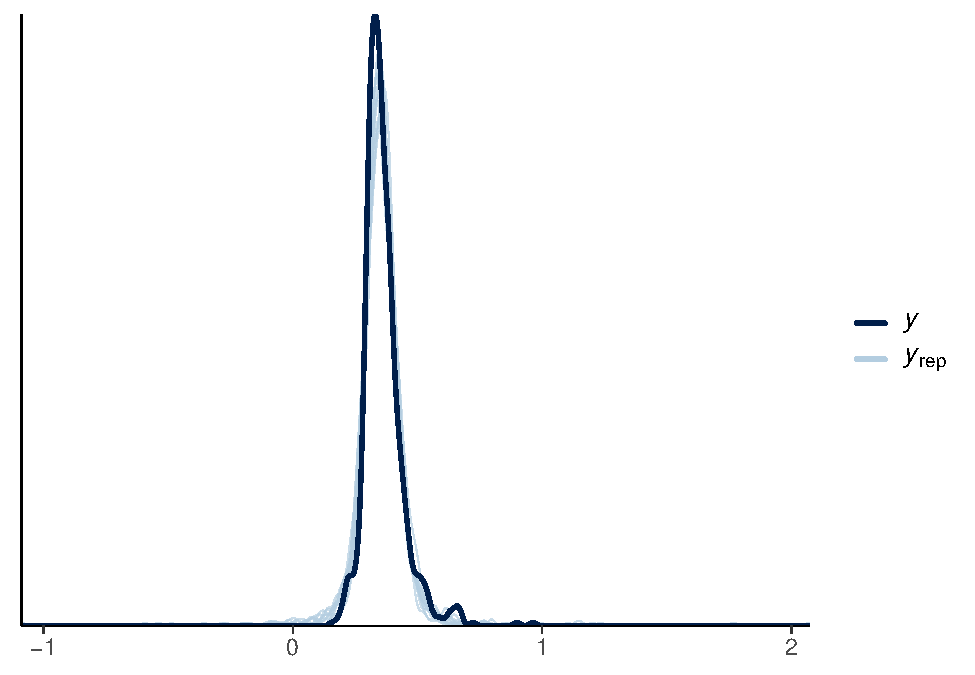
\includegraphics{params_analyses_files/figure-latex/unnamed-chunk-6-2.pdf}

\begin{Shaded}
\begin{Highlighting}[]
\FunctionTok{summary}\NormalTok{(m5)}
\end{Highlighting}
\end{Shaded}

\begin{verbatim}
## Warning: There were 5 divergent transitions after warmup. Increasing
## adapt_delta above 0.8 may help. See
## http://mc-stan.org/misc/warnings.html#divergent-transitions-after-warmup
\end{verbatim}

\begin{verbatim}
##  Family: student 
##   Links: mu = identity; sigma = identity; nu = identity 
## Formula: mu_ss ~ exp * blk + (1 + blk | subject) 
##    Data: df (Number of observations: 736) 
##   Draws: 4 chains, each with iter = 2000; warmup = 1000; thin = 1;
##          total post-warmup draws = 4000
## 
## Group-Level Effects: 
## ~subject (Number of levels: 184) 
##                     Estimate Est.Error l-95% CI u-95% CI Rhat Bulk_ESS Tail_ESS
## sd(Intercept)           0.03      0.00     0.03     0.04 1.01      955     1819
## sd(blk2)                0.01      0.01     0.00     0.03 1.01      465      870
## sd(blk3)                0.01      0.01     0.00     0.03 1.02      170      539
## sd(blk4)                0.02      0.01     0.00     0.04 1.01      278      447
## cor(Intercept,blk2)     0.34      0.35    -0.47     0.89 1.00     2039     2323
## cor(Intercept,blk3)    -0.16      0.38    -0.80     0.66 1.00     2011     2379
## cor(blk2,blk3)          0.09      0.44    -0.76     0.82 1.01      647     1778
## cor(Intercept,blk4)     0.32      0.29    -0.26     0.84 1.01      539     1783
## cor(blk2,blk4)          0.16      0.39    -0.64     0.82 1.01      481      912
## cor(blk3,blk4)          0.24      0.42    -0.66     0.87 1.02      297     1206
## 
## Population-Level Effects: 
##                  Estimate Est.Error l-95% CI u-95% CI Rhat Bulk_ESS Tail_ESS
## Intercept            0.34      0.01     0.33     0.36 1.01     1234     1736
## expsurprise         -0.01      0.01    -0.03     0.01 1.00     1351     1994
## blk2                 0.02      0.01     0.00     0.03 1.00     1596     1814
## blk3                 0.02      0.01     0.00     0.03 1.00     1766     1736
## blk4                 0.02      0.01     0.00     0.03 1.00     1484     1914
## expsurprise:blk2     0.00      0.01    -0.02     0.02 1.00     1855     2382
## expsurprise:blk3    -0.00      0.01    -0.02     0.02 1.00     1681     1772
## expsurprise:blk4     0.00      0.01    -0.02     0.02 1.00     1758     2166
## 
## Family Specific Parameters: 
##       Estimate Est.Error l-95% CI u-95% CI Rhat Bulk_ESS Tail_ESS
## sigma     0.03      0.00     0.03     0.04 1.01      400      576
## nu        2.22      0.29     1.72     2.86 1.00      808      724
## 
## Draws were sampled using sample(hmc). For each parameter, Bulk_ESS
## and Tail_ESS are effective sample size measures, and Rhat is the potential
## scale reduction factor on split chains (at convergence, Rhat = 1).
\end{verbatim}

\begin{Shaded}
\begin{Highlighting}[]
\FunctionTok{conditional\_effects}\NormalTok{(m5, }\StringTok{"blk:exp"}\NormalTok{)}
\end{Highlighting}
\end{Shaded}

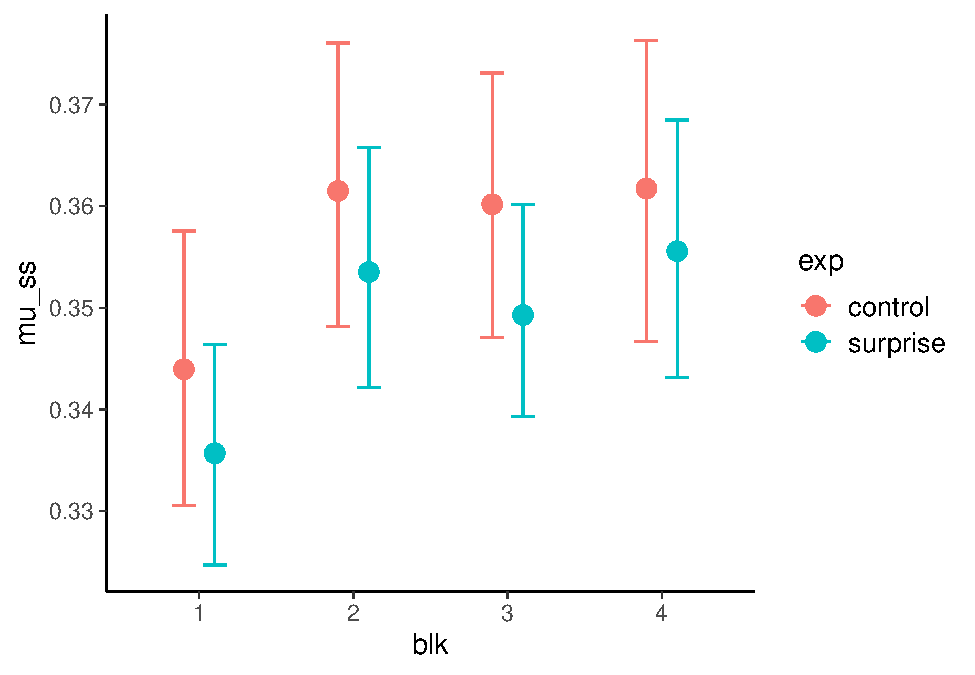
\includegraphics{params_analyses_files/figure-latex/unnamed-chunk-6-3.pdf}

Parameter mu\_rs2: Drift rate for phase 2 of response selection

\begin{Shaded}
\begin{Highlighting}[]
\FunctionTok{plot}\NormalTok{(}\FunctionTok{density}\NormalTok{(df}\SpecialCharTok{$}\NormalTok{mu\_rs2))}
\end{Highlighting}
\end{Shaded}

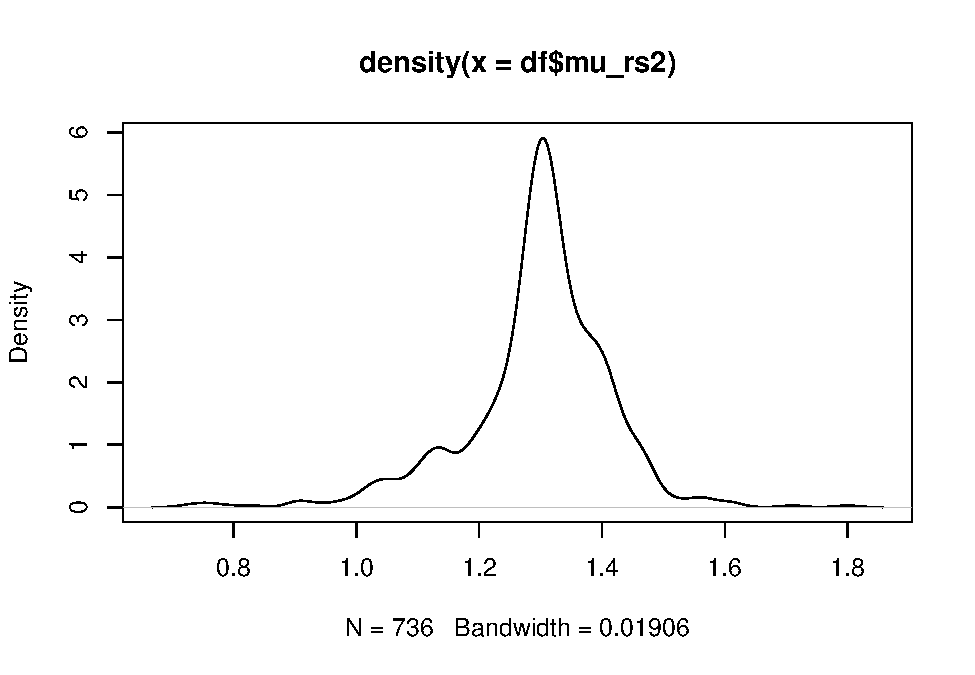
\includegraphics{params_analyses_files/figure-latex/unnamed-chunk-7-1.pdf}

\begin{Shaded}
\begin{Highlighting}[]
\NormalTok{m6 }\OtherTok{\textless{}{-}} \FunctionTok{brm}\NormalTok{(}
\NormalTok{  mu\_rs2 }\SpecialCharTok{\textasciitilde{}}\NormalTok{ exp }\SpecialCharTok{*}\NormalTok{ blk }\SpecialCharTok{+}\NormalTok{ (}\DecValTok{1} \SpecialCharTok{+}\NormalTok{ blk }\SpecialCharTok{|}\NormalTok{ subject),}
  \AttributeTok{family =} \FunctionTok{asym\_laplace}\NormalTok{(),}
  \AttributeTok{backend =} \StringTok{"cmdstanr"}\NormalTok{,}
  \CommentTok{\# algorithm = "meanfield",}
  \AttributeTok{data =}\NormalTok{ df}
\NormalTok{)}
\end{Highlighting}
\end{Shaded}

\begin{verbatim}
## In file included from /var/folders/cl/wwjrsxdd5tz7y9jr82nd5hrw0000gn/T/RtmpDVAVEa/model-d4401893cee9.hpp:1:
## In file included from /Users/corrado/.cmdstan/cmdstan-2.33.1/stan/src/stan/model/model_header.hpp:4:
## In file included from /Users/corrado/.cmdstan/cmdstan-2.33.1/stan/lib/stan_math/stan/math.hpp:19:
## In file included from /Users/corrado/.cmdstan/cmdstan-2.33.1/stan/lib/stan_math/stan/math/rev.hpp:10:
## In file included from /Users/corrado/.cmdstan/cmdstan-2.33.1/stan/lib/stan_math/stan/math/rev/fun.hpp:200:
## In file included from /Users/corrado/.cmdstan/cmdstan-2.33.1/stan/lib/stan_math/stan/math/prim/functor.hpp:16:
## In file included from /Users/corrado/.cmdstan/cmdstan-2.33.1/stan/lib/stan_math/stan/math/prim/functor/integrate_ode_rk45.hpp:6:
## In file included from /Users/corrado/.cmdstan/cmdstan-2.33.1/stan/lib/stan_math/stan/math/prim/functor/ode_rk45.hpp:9:
## In file included from /Users/corrado/.cmdstan/cmdstan-2.33.1/stan/lib/stan_math/lib/boost_1.78.0/boost/numeric/odeint.hpp:76:
## In file included from /Users/corrado/.cmdstan/cmdstan-2.33.1/stan/lib/stan_math/lib/boost_1.78.0/boost/numeric/odeint/integrate/observer_collection.hpp:23:
## In file included from /Users/corrado/.cmdstan/cmdstan-2.33.1/stan/lib/stan_math/lib/boost_1.78.0/boost/function.hpp:30:
## In file included from /Users/corrado/.cmdstan/cmdstan-2.33.1/stan/lib/stan_math/lib/boost_1.78.0/boost/function/detail/prologue.hpp:17:
## In file included from /Users/corrado/.cmdstan/cmdstan-2.33.1/stan/lib/stan_math/lib/boost_1.78.0/boost/function/function_base.hpp:21:
## In file included from /Users/corrado/.cmdstan/cmdstan-2.33.1/stan/lib/stan_math/lib/boost_1.78.0/boost/type_index.hpp:29:
## In file included from /Users/corrado/.cmdstan/cmdstan-2.33.1/stan/lib/stan_math/lib/boost_1.78.0/boost/type_index/stl_type_index.hpp:47:
## /Users/corrado/.cmdstan/cmdstan-2.33.1/stan/lib/stan_math/lib/boost_1.78.0/boost/container_hash/hash.hpp:132:33: warning: 'unary_function<const std::error_category *, unsigned long>' is deprecat
\end{verbatim}

\begin{verbatim}
## ed [-Wdeprecated-declarations]
##         struct hash_base : std::unary_function<T, std::size_t> {};
##                                 ^
## /Users/corrado/.cmdstan/cmdstan-2.33.1/stan/lib/stan_math/lib/boost_1.78.0/boost/container_hash/hash.hpp:692:18: note: in instantiation of template class 'boost::hash_detail::hash_base<const std::error_category *>' requested here
##         : public boost::hash_detail::hash_base<T*>
##                  ^
## /Users/corrado/.cmdstan/cmdstan-2.33.1/stan/lib/stan_math/lib/boost_1.78.0/boost/container_hash/hash.hpp:420:24: note: in instantiation of template class 'boost::hash<const std::error_category *>' requested here
##         boost::hash<T> hasher;
##                        ^
## /Users/corrado/.cmdstan/cmdstan-2.33.1/stan/lib/stan_math/lib/boost_1.78.0/boost/container_hash/hash.hpp:551:9: note: in instantiation of function template specialization 'boost::hash_combine<const std::error_category *>' requested here
##         hash_combine(seed, &v.category());
##         ^
\end{verbatim}

\begin{verbatim}
## /Library/Developer/CommandLineTools/SDKs/MacOSX.sdk/usr/include/c++/v1/__functional/unary_function.h:23:29: note: 'unary_function<const std::error_category *, unsigned long>' has been explicitly marked deprecated here
## struct _LIBCPP_TEMPLATE_VIS _LIBCPP_DEPRECATED_IN_CXX11 unary_function
##                             ^
## /Library/Developer/CommandLineTools/SDKs/MacOSX.sdk/usr/include/c++/v1/__config:825:41: note: expanded from macro '_LIBCPP_DEPRECATED_IN_CXX11'
## #    define _LIBCPP_DEPRECATED_IN_CXX11 _LIBCPP_DEPRECATED
##                                         ^
## /Library/Developer/CommandLineTools/SDKs/MacOSX.sdk/usr/include/c++/v1/__config:810:49: note: expanded from macro '_LIBCPP_DEPRECATED'
## #      define _LIBCPP_DEPRECATED __attribute__((deprecated))
##                                                 ^
\end{verbatim}

\begin{verbatim}
## 1 warning generated.
\end{verbatim}

\begin{verbatim}
## Start sampling
\end{verbatim}

\begin{verbatim}
## Running MCMC with 4 sequential chains...
## 
## Chain 1 Iteration:    1 / 2000 [  0%]  (Warmup) 
## Chain 1 Iteration:  100 / 2000 [  5%]  (Warmup) 
## Chain 1 Iteration:  200 / 2000 [ 10%]  (Warmup) 
## Chain 1 Iteration:  300 / 2000 [ 15%]  (Warmup) 
## Chain 1 Iteration:  400 / 2000 [ 20%]  (Warmup) 
## Chain 1 Iteration:  500 / 2000 [ 25%]  (Warmup) 
## Chain 1 Iteration:  600 / 2000 [ 30%]  (Warmup) 
## Chain 1 Iteration:  700 / 2000 [ 35%]  (Warmup) 
## Chain 1 Iteration:  800 / 2000 [ 40%]  (Warmup) 
## Chain 1 Iteration:  900 / 2000 [ 45%]  (Warmup) 
## Chain 1 Iteration: 1000 / 2000 [ 50%]  (Warmup) 
## Chain 1 Iteration: 1001 / 2000 [ 50%]  (Sampling) 
## Chain 1 Iteration: 1100 / 2000 [ 55%]  (Sampling) 
## Chain 1 Iteration: 1200 / 2000 [ 60%]  (Sampling) 
## Chain 1 Iteration: 1300 / 2000 [ 65%]  (Sampling) 
## Chain 1 Iteration: 1400 / 2000 [ 70%]  (Sampling) 
## Chain 1 Iteration: 1500 / 2000 [ 75%]  (Sampling) 
## Chain 1 Iteration: 1600 / 2000 [ 80%]  (Sampling) 
## Chain 1 Iteration: 1700 / 2000 [ 85%]  (Sampling) 
## Chain 1 Iteration: 1800 / 2000 [ 90%]  (Sampling) 
## Chain 1 Iteration: 1900 / 2000 [ 95%]  (Sampling) 
## Chain 1 Iteration: 2000 / 2000 [100%]  (Sampling) 
## Chain 1 finished in 37.0 seconds.
## Chain 2 Iteration:    1 / 2000 [  0%]  (Warmup) 
## Chain 2 Iteration:  100 / 2000 [  5%]  (Warmup) 
## Chain 2 Iteration:  200 / 2000 [ 10%]  (Warmup) 
## Chain 2 Iteration:  300 / 2000 [ 15%]  (Warmup) 
## Chain 2 Iteration:  400 / 2000 [ 20%]  (Warmup) 
## Chain 2 Iteration:  500 / 2000 [ 25%]  (Warmup) 
## Chain 2 Iteration:  600 / 2000 [ 30%]  (Warmup) 
## Chain 2 Iteration:  700 / 2000 [ 35%]  (Warmup) 
## Chain 2 Iteration:  800 / 2000 [ 40%]  (Warmup) 
## Chain 2 Iteration:  900 / 2000 [ 45%]  (Warmup) 
## Chain 2 Iteration: 1000 / 2000 [ 50%]  (Warmup) 
## Chain 2 Iteration: 1001 / 2000 [ 50%]  (Sampling) 
## Chain 2 Iteration: 1100 / 2000 [ 55%]  (Sampling) 
## Chain 2 Iteration: 1200 / 2000 [ 60%]  (Sampling) 
## Chain 2 Iteration: 1300 / 2000 [ 65%]  (Sampling) 
## Chain 2 Iteration: 1400 / 2000 [ 70%]  (Sampling) 
## Chain 2 Iteration: 1500 / 2000 [ 75%]  (Sampling) 
## Chain 2 Iteration: 1600 / 2000 [ 80%]  (Sampling) 
## Chain 2 Iteration: 1700 / 2000 [ 85%]  (Sampling) 
## Chain 2 Iteration: 1800 / 2000 [ 90%]  (Sampling) 
## Chain 2 Iteration: 1900 / 2000 [ 95%]  (Sampling) 
## Chain 2 Iteration: 2000 / 2000 [100%]  (Sampling) 
## Chain 2 finished in 30.2 seconds.
## Chain 3 Iteration:    1 / 2000 [  0%]  (Warmup) 
## Chain 3 Iteration:  100 / 2000 [  5%]  (Warmup) 
## Chain 3 Iteration:  200 / 2000 [ 10%]  (Warmup) 
## Chain 3 Iteration:  300 / 2000 [ 15%]  (Warmup) 
## Chain 3 Iteration:  400 / 2000 [ 20%]  (Warmup) 
## Chain 3 Iteration:  500 / 2000 [ 25%]  (Warmup) 
## Chain 3 Iteration:  600 / 2000 [ 30%]  (Warmup) 
## Chain 3 Iteration:  700 / 2000 [ 35%]  (Warmup) 
## Chain 3 Iteration:  800 / 2000 [ 40%]  (Warmup) 
## Chain 3 Iteration:  900 / 2000 [ 45%]  (Warmup) 
## Chain 3 Iteration: 1000 / 2000 [ 50%]  (Warmup) 
## Chain 3 Iteration: 1001 / 2000 [ 50%]  (Sampling) 
## Chain 3 Iteration: 1100 / 2000 [ 55%]  (Sampling) 
## Chain 3 Iteration: 1200 / 2000 [ 60%]  (Sampling) 
## Chain 3 Iteration: 1300 / 2000 [ 65%]  (Sampling) 
## Chain 3 Iteration: 1400 / 2000 [ 70%]  (Sampling) 
## Chain 3 Iteration: 1500 / 2000 [ 75%]  (Sampling) 
## Chain 3 Iteration: 1600 / 2000 [ 80%]  (Sampling) 
## Chain 3 Iteration: 1700 / 2000 [ 85%]  (Sampling) 
## Chain 3 Iteration: 1800 / 2000 [ 90%]  (Sampling) 
## Chain 3 Iteration: 1900 / 2000 [ 95%]  (Sampling) 
## Chain 3 Iteration: 2000 / 2000 [100%]  (Sampling) 
## Chain 3 finished in 28.8 seconds.
## Chain 4 Iteration:    1 / 2000 [  0%]  (Warmup) 
## Chain 4 Iteration:  100 / 2000 [  5%]  (Warmup) 
## Chain 4 Iteration:  200 / 2000 [ 10%]  (Warmup) 
## Chain 4 Iteration:  300 / 2000 [ 15%]  (Warmup) 
## Chain 4 Iteration:  400 / 2000 [ 20%]  (Warmup) 
## Chain 4 Iteration:  500 / 2000 [ 25%]  (Warmup) 
## Chain 4 Iteration:  600 / 2000 [ 30%]  (Warmup) 
## Chain 4 Iteration:  700 / 2000 [ 35%]  (Warmup) 
## Chain 4 Iteration:  800 / 2000 [ 40%]  (Warmup) 
## Chain 4 Iteration:  900 / 2000 [ 45%]  (Warmup) 
## Chain 4 Iteration: 1000 / 2000 [ 50%]  (Warmup) 
## Chain 4 Iteration: 1001 / 2000 [ 50%]  (Sampling) 
## Chain 4 Iteration: 1100 / 2000 [ 55%]  (Sampling) 
## Chain 4 Iteration: 1200 / 2000 [ 60%]  (Sampling) 
## Chain 4 Iteration: 1300 / 2000 [ 65%]  (Sampling) 
## Chain 4 Iteration: 1400 / 2000 [ 70%]  (Sampling) 
## Chain 4 Iteration: 1500 / 2000 [ 75%]  (Sampling) 
## Chain 4 Iteration: 1600 / 2000 [ 80%]  (Sampling) 
## Chain 4 Iteration: 1700 / 2000 [ 85%]  (Sampling) 
## Chain 4 Iteration: 1800 / 2000 [ 90%]  (Sampling) 
## Chain 4 Iteration: 1900 / 2000 [ 95%]  (Sampling) 
## Chain 4 Iteration: 2000 / 2000 [100%]  (Sampling) 
## Chain 4 finished in 37.4 seconds.
## 
## All 4 chains finished successfully.
## Mean chain execution time: 33.3 seconds.
## Total execution time: 133.6 seconds.
\end{verbatim}

\begin{Shaded}
\begin{Highlighting}[]
\FunctionTok{pp\_check}\NormalTok{(m6)}
\end{Highlighting}
\end{Shaded}

\begin{verbatim}
## Using 10 posterior draws for ppc type 'dens_overlay' by default.
\end{verbatim}

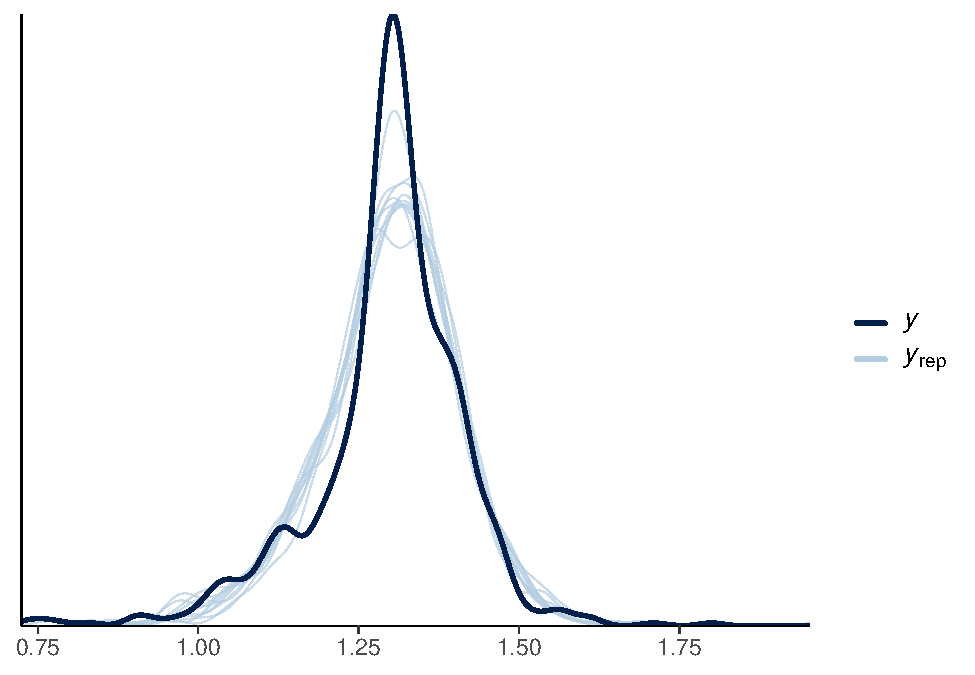
\includegraphics{params_analyses_files/figure-latex/unnamed-chunk-7-2.pdf}

\begin{Shaded}
\begin{Highlighting}[]
\FunctionTok{summary}\NormalTok{(m6)}
\end{Highlighting}
\end{Shaded}

\begin{verbatim}
##  Family: asym_laplace 
##   Links: mu = identity; sigma = identity; quantile = identity 
## Formula: mu_rs2 ~ exp * blk + (1 + blk | subject) 
##    Data: df (Number of observations: 736) 
##   Draws: 4 chains, each with iter = 2000; warmup = 1000; thin = 1;
##          total post-warmup draws = 4000
## 
## Group-Level Effects: 
## ~subject (Number of levels: 184) 
##                     Estimate Est.Error l-95% CI u-95% CI Rhat Bulk_ESS Tail_ESS
## sd(Intercept)           0.06      0.01     0.05     0.07 1.00      912     1423
## sd(blk2)                0.01      0.01     0.00     0.03 1.00      881     1339
## sd(blk3)                0.01      0.01     0.00     0.03 1.00      996      954
## sd(blk4)                0.01      0.01     0.00     0.04 1.01      538     1025
## cor(Intercept,blk2)     0.09      0.42    -0.75     0.82 1.00     3006     2342
## cor(Intercept,blk3)    -0.01      0.44    -0.81     0.78 1.00     3165     2255
## cor(blk2,blk3)          0.09      0.45    -0.77     0.84 1.00     1837     2743
## cor(Intercept,blk4)    -0.15      0.39    -0.80     0.68 1.00     2379     2232
## cor(blk2,blk4)          0.06      0.45    -0.77     0.85 1.00     1216     1572
## cor(blk3,blk4)          0.10      0.45    -0.77     0.87 1.00     1215     1638
## 
## Population-Level Effects: 
##                  Estimate Est.Error l-95% CI u-95% CI Rhat Bulk_ESS Tail_ESS
## Intercept            1.33      0.01     1.31     1.36 1.01      862     1865
## expsurprise         -0.00      0.01    -0.03     0.03 1.00      998     1515
## blk2                -0.02      0.01    -0.04     0.00 1.00     1446     2594
## blk3                -0.01      0.01    -0.04     0.01 1.00     1236     2388
## blk4                -0.02      0.01    -0.04     0.00 1.00     1546     2468
## expsurprise:blk2     0.01      0.02    -0.02     0.04 1.00     1485     2641
## expsurprise:blk3    -0.01      0.02    -0.04     0.02 1.00     1274     2090
## expsurprise:blk4     0.01      0.02    -0.02     0.04 1.00     1389     2325
## 
## Family Specific Parameters: 
##          Estimate Est.Error l-95% CI u-95% CI Rhat Bulk_ESS Tail_ESS
## sigma        0.03      0.00     0.03     0.03 1.00     1727     2350
## quantile     0.59      0.03     0.54     0.64 1.00     1431     2264
## 
## Draws were sampled using sample(hmc). For each parameter, Bulk_ESS
## and Tail_ESS are effective sample size measures, and Rhat is the potential
## scale reduction factor on split chains (at convergence, Rhat = 1).
\end{verbatim}

\begin{Shaded}
\begin{Highlighting}[]
\FunctionTok{conditional\_effects}\NormalTok{(m6, }\StringTok{"blk:exp"}\NormalTok{)}
\end{Highlighting}
\end{Shaded}

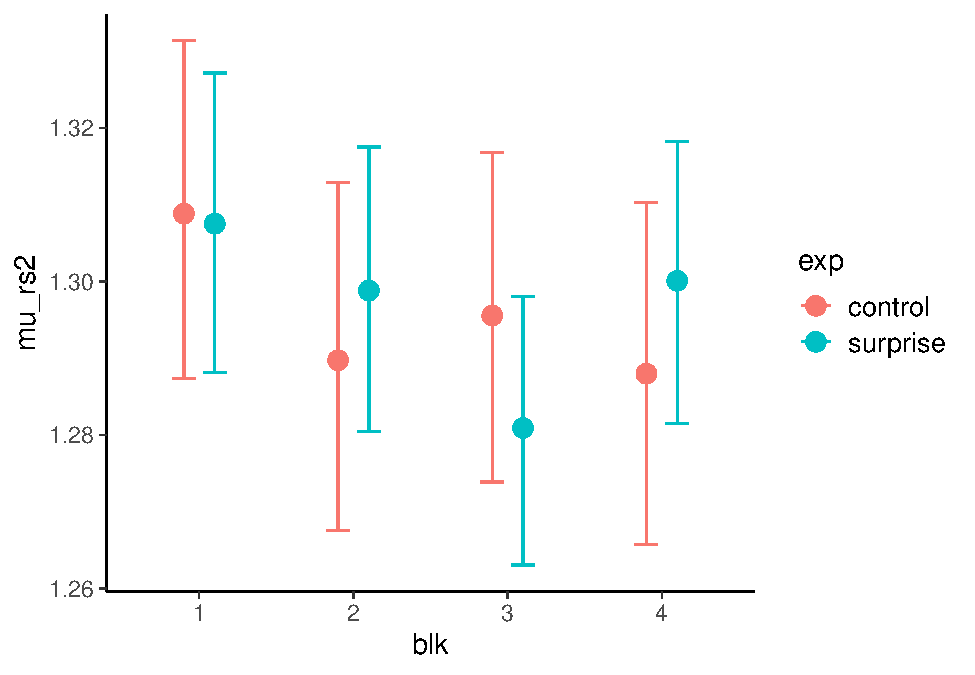
\includegraphics{params_analyses_files/figure-latex/unnamed-chunk-7-3.pdf}

Parameter ter: Drift rate for phase 2 of response selection

\begin{Shaded}
\begin{Highlighting}[]
\FunctionTok{plot}\NormalTok{(}\FunctionTok{density}\NormalTok{(df}\SpecialCharTok{$}\NormalTok{ter))}
\end{Highlighting}
\end{Shaded}

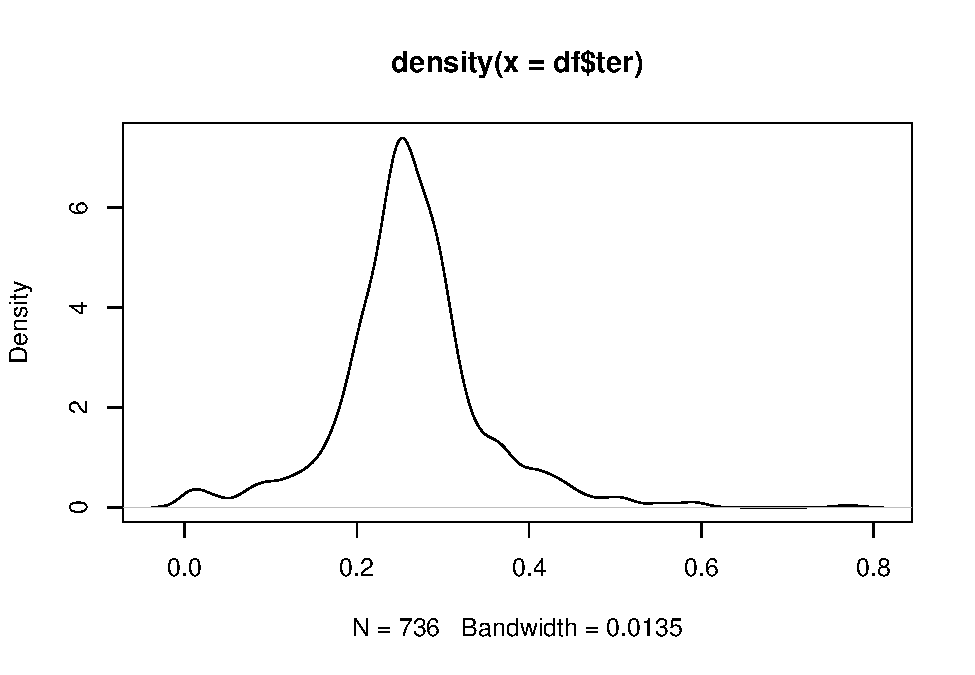
\includegraphics{params_analyses_files/figure-latex/unnamed-chunk-8-1.pdf}

\begin{Shaded}
\begin{Highlighting}[]
\NormalTok{m7 }\OtherTok{\textless{}{-}} \FunctionTok{brm}\NormalTok{(}
\NormalTok{  ter }\SpecialCharTok{\textasciitilde{}}\NormalTok{ exp }\SpecialCharTok{*}\NormalTok{ blk }\SpecialCharTok{+}\NormalTok{ (}\DecValTok{1} \SpecialCharTok{+}\NormalTok{ blk }\SpecialCharTok{|}\NormalTok{ subject),}
  \AttributeTok{family =} \FunctionTok{asym\_laplace}\NormalTok{(),}
  \AttributeTok{backend =} \StringTok{"cmdstanr"}\NormalTok{,}
  \CommentTok{\# algorithm = "meanfield",}
  \AttributeTok{data =}\NormalTok{ df}
\NormalTok{)}
\end{Highlighting}
\end{Shaded}

\begin{verbatim}
## In file included from /var/folders/cl/wwjrsxdd5tz7y9jr82nd5hrw0000gn/T/RtmpDVAVEa/model-d4405e73239b.hpp:1:
## In file included from /Users/corrado/.cmdstan/cmdstan-2.33.1/stan/src/stan/model/model_header.hpp:4:
## In file included from /Users/corrado/.cmdstan/cmdstan-2.33.1/stan/lib/stan_math/stan/math.hpp:19:
## In file included from /Users/corrado/.cmdstan/cmdstan-2.33.1/stan/lib/stan_math/stan/math/rev.hpp:10:
## In file included from /Users/corrado/.cmdstan/cmdstan-2.33.1/stan/lib/stan_math/stan/math/rev/fun.hpp:200:
## In file included from /Users/corrado/.cmdstan/cmdstan-2.33.1/stan/lib/stan_math/stan/math/prim/functor.hpp:16:
## In file included from /Users/corrado/.cmdstan/cmdstan-2.33.1/stan/lib/stan_math/stan/math/prim/functor/integrate_ode_rk45.hpp:6:
## In file included from /Users/corrado/.cmdstan/cmdstan-2.33.1/stan/lib/stan_math/stan/math/prim/functor/ode_rk45.hpp:9:
## In file included from /Users/corrado/.cmdstan/cmdstan-2.33.1/stan/lib/stan_math/lib/boost_1.78.0/boost/numeric/odeint.hpp:76:
## In file included from /Users/corrado/.cmdstan/cmdstan-2.33.1/stan/lib/stan_math/lib/boost_1.78.0/boost/numeric/odeint/integrate/observer_collection.hpp:23:
## In file included from /Users/corrado/.cmdstan/cmdstan-2.33.1/stan/lib/stan_math/lib/boost_1.78.0/boost/function.hpp:30:
## In file included from /Users/corrado/.cmdstan/cmdstan-2.33.1/stan/lib/stan_math/lib/boost_1.78.0/boost/function/detail/prologue.hpp:17:
## In file included from /Users/corrado/.cmdstan/cmdstan-2.33.1/stan/lib/stan_math/lib/boost_1.78.0/boost/function/function_base.hpp:21:
## In file included from /Users/corrado/.cmdstan/cmdstan-2.33.1/stan/lib/stan_math/lib/boost_1.78.0/boost/type_index.hpp:29:
## In file included from /Users/corrado/.cmdstan/cmdstan-2.33.1/stan/lib/stan_math/lib/boost_1.78.0/boost/type_index/stl_type_index.hpp:47:
## /Users/corrado/.cmdstan/cmdstan-2.33.1/stan/lib/stan_math/lib/boost_1.78.0/boost/container_hash/hash.hpp:132:33: warning: 'unary_function<const std::error_category *, unsigned long>' is deprecat
\end{verbatim}

\begin{verbatim}
## ed [-Wdeprecated-declarations]
##         struct hash_base : std::unary_function<T, std::size_t> {};
##                                 ^
## /Users/corrado/.cmdstan/cmdstan-2.33.1/stan/lib/stan_math/lib/boost_1.78.0/boost/container_hash/hash.hpp:692:18: note: in instantiation of template class 'boost::hash_detail::hash_base<const std::error_category *>' requested here
##         : public boost::hash_detail::hash_base<T*>
##                  ^
## /Users/corrado/.cmdstan/cmdstan-2.33.1/stan/lib/stan_math/lib/boost_1.78.0/boost/container_hash/hash.hpp:420:24: note: in instantiation of template class 'boost::hash<const std::error_category *>' requested here
##         boost::hash<T> hasher;
##                        ^
## /Users/corrado/.cmdstan/cmdstan-2.33.1/stan/lib/stan_math/lib/boost_1.78.0/boost/container_hash/hash.hpp:551:9: note: in instantiation of function template specialization 'boost::hash_combine<const std::error_category *>' requested here
##         hash_combine(seed, &v.category());
##         ^
\end{verbatim}

\begin{verbatim}
## /Library/Developer/CommandLineTools/SDKs/MacOSX.sdk/usr/include/c++/v1/__functional/unary_function.h:23:29: note: 'unary_function<const std::error_category *, unsigned long>' has been explicitly marked deprecated here
## struct _LIBCPP_TEMPLATE_VIS _LIBCPP_DEPRECATED_IN_CXX11 unary_function
##                             ^
## /Library/Developer/CommandLineTools/SDKs/MacOSX.sdk/usr/include/c++/v1/__config:825:41: note: expanded from macro '_LIBCPP_DEPRECATED_IN_CXX11'
## #    define _LIBCPP_DEPRECATED_IN_CXX11 _LIBCPP_DEPRECATED
##                                         ^
## /Library/Developer/CommandLineTools/SDKs/MacOSX.sdk/usr/include/c++/v1/__config:810:49: note: expanded from macro '_LIBCPP_DEPRECATED'
## #      define _LIBCPP_DEPRECATED __attribute__((deprecated))
##                                                 ^
\end{verbatim}

\begin{verbatim}
## 1 warning generated.
\end{verbatim}

\begin{verbatim}
## Start sampling
\end{verbatim}

\begin{verbatim}
## Running MCMC with 4 sequential chains...
## 
## Chain 1 Iteration:    1 / 2000 [  0%]  (Warmup) 
## Chain 1 Iteration:  100 / 2000 [  5%]  (Warmup) 
## Chain 1 Iteration:  200 / 2000 [ 10%]  (Warmup) 
## Chain 1 Iteration:  300 / 2000 [ 15%]  (Warmup) 
## Chain 1 Iteration:  400 / 2000 [ 20%]  (Warmup) 
## Chain 1 Iteration:  500 / 2000 [ 25%]  (Warmup) 
## Chain 1 Iteration:  600 / 2000 [ 30%]  (Warmup) 
## Chain 1 Iteration:  700 / 2000 [ 35%]  (Warmup) 
## Chain 1 Iteration:  800 / 2000 [ 40%]  (Warmup) 
## Chain 1 Iteration:  900 / 2000 [ 45%]  (Warmup) 
## Chain 1 Iteration: 1000 / 2000 [ 50%]  (Warmup) 
## Chain 1 Iteration: 1001 / 2000 [ 50%]  (Sampling) 
## Chain 1 Iteration: 1100 / 2000 [ 55%]  (Sampling) 
## Chain 1 Iteration: 1200 / 2000 [ 60%]  (Sampling) 
## Chain 1 Iteration: 1300 / 2000 [ 65%]  (Sampling) 
## Chain 1 Iteration: 1400 / 2000 [ 70%]  (Sampling) 
## Chain 1 Iteration: 1500 / 2000 [ 75%]  (Sampling) 
## Chain 1 Iteration: 1600 / 2000 [ 80%]  (Sampling) 
## Chain 1 Iteration: 1700 / 2000 [ 85%]  (Sampling) 
## Chain 1 Iteration: 1800 / 2000 [ 90%]  (Sampling) 
## Chain 1 Iteration: 1900 / 2000 [ 95%]  (Sampling) 
## Chain 1 Iteration: 2000 / 2000 [100%]  (Sampling) 
## Chain 1 finished in 44.5 seconds.
## Chain 2 Iteration:    1 / 2000 [  0%]  (Warmup) 
## Chain 2 Iteration:  100 / 2000 [  5%]  (Warmup) 
## Chain 2 Iteration:  200 / 2000 [ 10%]  (Warmup) 
## Chain 2 Iteration:  300 / 2000 [ 15%]  (Warmup) 
## Chain 2 Iteration:  400 / 2000 [ 20%]  (Warmup) 
## Chain 2 Iteration:  500 / 2000 [ 25%]  (Warmup) 
## Chain 2 Iteration:  600 / 2000 [ 30%]  (Warmup) 
## Chain 2 Iteration:  700 / 2000 [ 35%]  (Warmup) 
## Chain 2 Iteration:  800 / 2000 [ 40%]  (Warmup) 
## Chain 2 Iteration:  900 / 2000 [ 45%]  (Warmup) 
## Chain 2 Iteration: 1000 / 2000 [ 50%]  (Warmup) 
## Chain 2 Iteration: 1001 / 2000 [ 50%]  (Sampling) 
## Chain 2 Iteration: 1100 / 2000 [ 55%]  (Sampling) 
## Chain 2 Iteration: 1200 / 2000 [ 60%]  (Sampling) 
## Chain 2 Iteration: 1300 / 2000 [ 65%]  (Sampling) 
## Chain 2 Iteration: 1400 / 2000 [ 70%]  (Sampling) 
## Chain 2 Iteration: 1500 / 2000 [ 75%]  (Sampling) 
## Chain 2 Iteration: 1600 / 2000 [ 80%]  (Sampling) 
## Chain 2 Iteration: 1700 / 2000 [ 85%]  (Sampling) 
## Chain 2 Iteration: 1800 / 2000 [ 90%]  (Sampling) 
## Chain 2 Iteration: 1900 / 2000 [ 95%]  (Sampling) 
## Chain 2 Iteration: 2000 / 2000 [100%]  (Sampling) 
## Chain 2 finished in 41.1 seconds.
## Chain 3 Iteration:    1 / 2000 [  0%]  (Warmup) 
## Chain 3 Iteration:  100 / 2000 [  5%]  (Warmup) 
## Chain 3 Iteration:  200 / 2000 [ 10%]  (Warmup) 
## Chain 3 Iteration:  300 / 2000 [ 15%]  (Warmup) 
## Chain 3 Iteration:  400 / 2000 [ 20%]  (Warmup) 
## Chain 3 Iteration:  500 / 2000 [ 25%]  (Warmup) 
## Chain 3 Iteration:  600 / 2000 [ 30%]  (Warmup) 
## Chain 3 Iteration:  700 / 2000 [ 35%]  (Warmup) 
## Chain 3 Iteration:  800 / 2000 [ 40%]  (Warmup) 
## Chain 3 Iteration:  900 / 2000 [ 45%]  (Warmup) 
## Chain 3 Iteration: 1000 / 2000 [ 50%]  (Warmup) 
## Chain 3 Iteration: 1001 / 2000 [ 50%]  (Sampling) 
## Chain 3 Iteration: 1100 / 2000 [ 55%]  (Sampling) 
## Chain 3 Iteration: 1200 / 2000 [ 60%]  (Sampling) 
## Chain 3 Iteration: 1300 / 2000 [ 65%]  (Sampling) 
## Chain 3 Iteration: 1400 / 2000 [ 70%]  (Sampling) 
## Chain 3 Iteration: 1500 / 2000 [ 75%]  (Sampling) 
## Chain 3 Iteration: 1600 / 2000 [ 80%]  (Sampling) 
## Chain 3 Iteration: 1700 / 2000 [ 85%]  (Sampling) 
## Chain 3 Iteration: 1800 / 2000 [ 90%]  (Sampling) 
## Chain 3 Iteration: 1900 / 2000 [ 95%]  (Sampling) 
## Chain 3 Iteration: 2000 / 2000 [100%]  (Sampling) 
## Chain 3 finished in 46.4 seconds.
## Chain 4 Iteration:    1 / 2000 [  0%]  (Warmup) 
## Chain 4 Iteration:  100 / 2000 [  5%]  (Warmup) 
## Chain 4 Iteration:  200 / 2000 [ 10%]  (Warmup) 
## Chain 4 Iteration:  300 / 2000 [ 15%]  (Warmup) 
## Chain 4 Iteration:  400 / 2000 [ 20%]  (Warmup) 
## Chain 4 Iteration:  500 / 2000 [ 25%]  (Warmup) 
## Chain 4 Iteration:  600 / 2000 [ 30%]  (Warmup) 
## Chain 4 Iteration:  700 / 2000 [ 35%]  (Warmup) 
## Chain 4 Iteration:  800 / 2000 [ 40%]  (Warmup) 
## Chain 4 Iteration:  900 / 2000 [ 45%]  (Warmup) 
## Chain 4 Iteration: 1000 / 2000 [ 50%]  (Warmup) 
## Chain 4 Iteration: 1001 / 2000 [ 50%]  (Sampling) 
## Chain 4 Iteration: 1100 / 2000 [ 55%]  (Sampling) 
## Chain 4 Iteration: 1200 / 2000 [ 60%]  (Sampling) 
## Chain 4 Iteration: 1300 / 2000 [ 65%]  (Sampling) 
## Chain 4 Iteration: 1400 / 2000 [ 70%]  (Sampling) 
## Chain 4 Iteration: 1500 / 2000 [ 75%]  (Sampling) 
## Chain 4 Iteration: 1600 / 2000 [ 80%]  (Sampling) 
## Chain 4 Iteration: 1700 / 2000 [ 85%]  (Sampling) 
## Chain 4 Iteration: 1800 / 2000 [ 90%]  (Sampling) 
## Chain 4 Iteration: 1900 / 2000 [ 95%]  (Sampling) 
## Chain 4 Iteration: 2000 / 2000 [100%]  (Sampling) 
## Chain 4 finished in 40.0 seconds.
## 
## All 4 chains finished successfully.
## Mean chain execution time: 43.0 seconds.
## Total execution time: 172.3 seconds.
\end{verbatim}

\begin{Shaded}
\begin{Highlighting}[]
\FunctionTok{pp\_check}\NormalTok{(m7)}
\end{Highlighting}
\end{Shaded}

\begin{verbatim}
## Using 10 posterior draws for ppc type 'dens_overlay' by default.
\end{verbatim}

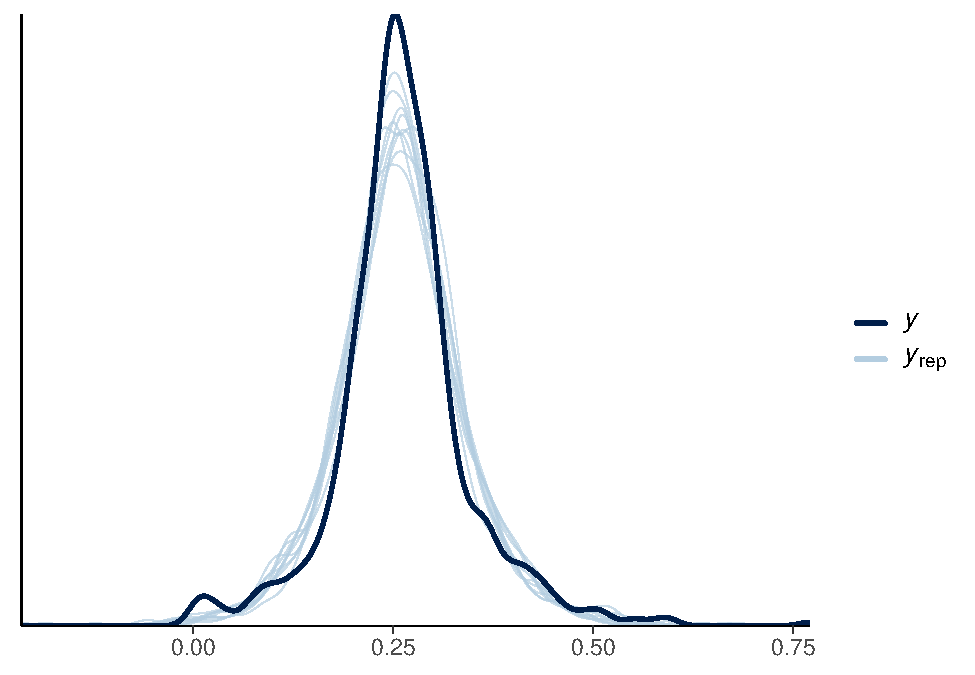
\includegraphics{params_analyses_files/figure-latex/unnamed-chunk-8-2.pdf}

\begin{Shaded}
\begin{Highlighting}[]
\FunctionTok{summary}\NormalTok{(m7)}
\end{Highlighting}
\end{Shaded}

\begin{verbatim}
##  Family: asym_laplace 
##   Links: mu = identity; sigma = identity; quantile = identity 
## Formula: ter ~ exp * blk + (1 + blk | subject) 
##    Data: df (Number of observations: 736) 
##   Draws: 4 chains, each with iter = 2000; warmup = 1000; thin = 1;
##          total post-warmup draws = 4000
## 
## Group-Level Effects: 
## ~subject (Number of levels: 184) 
##                     Estimate Est.Error l-95% CI u-95% CI Rhat Bulk_ESS Tail_ESS
## sd(Intercept)           0.05      0.01     0.04     0.06 1.01      586      766
## sd(blk2)                0.01      0.01     0.00     0.03 1.01      776     1650
## sd(blk3)                0.01      0.01     0.00     0.03 1.01      439      491
## sd(blk4)                0.02      0.01     0.00     0.04 1.01      394      473
## cor(Intercept,blk2)     0.41      0.34    -0.38     0.91 1.00     1487     2562
## cor(Intercept,blk3)    -0.30      0.40    -0.88     0.64 1.00     1860     2405
## cor(blk2,blk3)          0.02      0.44    -0.80     0.80 1.00     1153     2280
## cor(Intercept,blk4)    -0.53      0.31    -0.91     0.34 1.00     2374     1795
## cor(blk2,blk4)         -0.09      0.41    -0.82     0.71 1.00      826     1549
## cor(blk3,blk4)          0.34      0.45    -0.66     0.95 1.01      678     1413
## 
## Population-Level Effects: 
##                  Estimate Est.Error l-95% CI u-95% CI Rhat Bulk_ESS Tail_ESS
## Intercept            0.25      0.01     0.23     0.27 1.00     1336     2332
## expsurprise          0.02      0.01    -0.00     0.04 1.00     1155     2114
## blk2                 0.01      0.01    -0.00     0.03 1.00     2706     3087
## blk3                 0.01      0.01    -0.01     0.03 1.00     2053     2721
## blk4                 0.02      0.01    -0.00     0.03 1.00     2154     3000
## expsurprise:blk2    -0.01      0.01    -0.03     0.01 1.00     2566     2799
## expsurprise:blk3    -0.01      0.01    -0.03     0.01 1.00     1842     2281
## expsurprise:blk4    -0.02      0.01    -0.05     0.00 1.00     1729     2655
## 
## Family Specific Parameters: 
##          Estimate Est.Error l-95% CI u-95% CI Rhat Bulk_ESS Tail_ESS
## sigma        0.02      0.00     0.02     0.02 1.01     1019     1710
## quantile     0.52      0.03     0.47     0.58 1.00     1470     2001
## 
## Draws were sampled using sample(hmc). For each parameter, Bulk_ESS
## and Tail_ESS are effective sample size measures, and Rhat is the potential
## scale reduction factor on split chains (at convergence, Rhat = 1).
\end{verbatim}

\begin{Shaded}
\begin{Highlighting}[]
\FunctionTok{conditional\_effects}\NormalTok{(m7, }\StringTok{"blk:exp"}\NormalTok{)}
\end{Highlighting}
\end{Shaded}

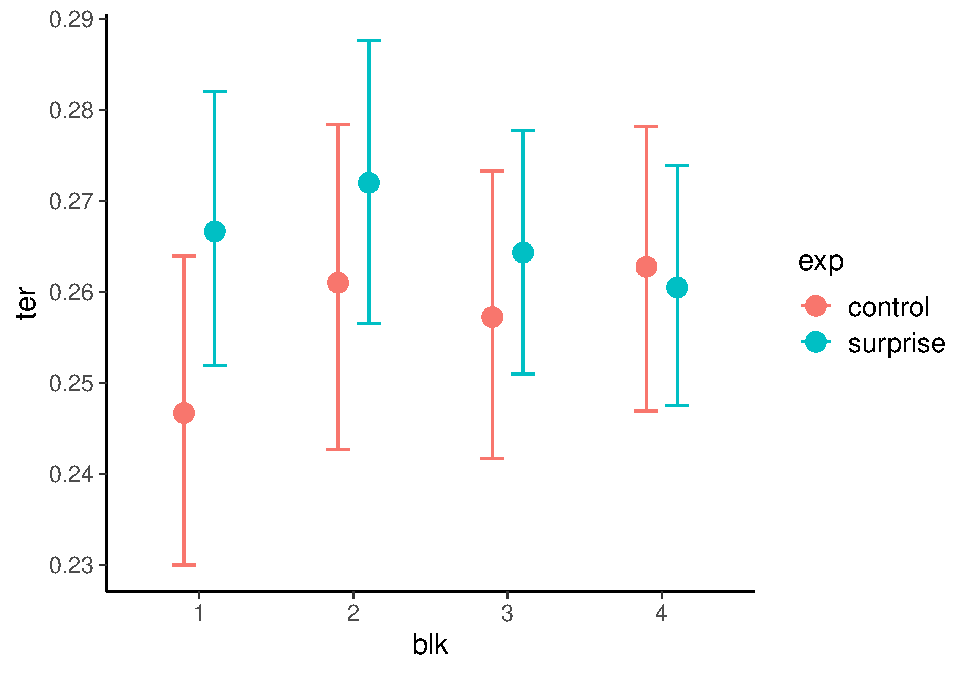
\includegraphics{params_analyses_files/figure-latex/unnamed-chunk-8-3.pdf}

\end{document}
